\documentclass[11pt]{aghdpl}
% \documentclass[en,11pt]{aghdpl}  % praca w języku angielskim

% Lista wszystkich języków stanowiących języki pozycji bibliograficznych użytych w pracy.
% (Zgodnie z zasadami tworzenia bibliografii każda pozycja powinna zostać utworzona zgodnie z zasadami języka, w którym dana publikacja została napisana.)
\usepackage[english,polish]{babel}

% Użyj polskiego łamania wyrazów (zamiast domyślnego angielskiego).
\usepackage{polski}

\usepackage[utf8]{inputenc}

% dodatkowe pakiety

\usepackage{mathtools}
\usepackage{amsfonts}
\usepackage{amsmath}
\usepackage{amsthm}

% --- < bibliografia > ---

\usepackage[
style=numeric,
sorting=none,
%
% Zastosuj styl wpisu bibliograficznego właściwy językowi publikacji.
language=autobib,
autolang=other,
% Zapisuj datę dostępu do strony WWW w formacie RRRR-MM-DD.
urldate=iso8601,
% Nie dodawaj numerów stron, na których występuje cytowanie.
backref=false,
% Podawaj ISBN.
isbn=true,
% Nie podawaj URL-i, o ile nie jest to konieczne.
url=false,
%
% Ustawienia związane z polskimi normami dla bibliografii.
maxbibnames=3,
% Jeżeli używamy BibTeXa:
backend=bibtex
]{biblatex}

\usepackage{csquotes}
% Ponieważ `csquotes` nie posiada polskiego stylu, można skorzystać z mocno zbliżonego stylu chorwackiego.
\DeclareQuoteAlias{croatian}{polish}

\addbibresource{bibliografia.bib}

% Nie wyświetlaj wybranych pól.
%\AtEveryBibitem{\clearfield{note}}


% ------------------------
% --- < listingi > ---

% Użyj czcionki kroju Courier.
\usepackage{courier}

\usepackage{listings}
\lstloadlanguages{TeX}

\lstset{
	literate={ą}{{\k{a}}}1
           {ć}{{\'c}}1
           {ę}{{\k{e}}}1
           {ó}{{\'o}}1
           {ń}{{\'n}}1
           {ł}{{\l{}}}1
           {ś}{{\'s}}1
           {ź}{{\'z}}1
           {ż}{{\.z}}1
           {Ą}{{\k{A}}}1
           {Ć}{{\'C}}1
           {Ę}{{\k{E}}}1
           {Ó}{{\'O}}1
           {Ń}{{\'N}}1
           {Ł}{{\L{}}}1
           {Ś}{{\'S}}1
           {Ź}{{\'Z}}1
           {Ż}{{\.Z}}1,
	basicstyle=\footnotesize\ttfamily,
}

% ------------------------

\AtBeginDocument{
	\renewcommand{\tablename}{Tabela}
	\renewcommand{\figurename}{Rys.}
}

% ------------------------
% --- < tabele > ---

\usepackage{array}
\usepackage{tabularx}
\usepackage{multirow}
\usepackage{booktabs}
\usepackage{makecell}
\usepackage[flushleft]{threeparttable}

% defines the X column to use m (\parbox[c]) instead of p (`parbox[t]`)
\newcolumntype{C}[1]{>{\hsize=#1\hsize\centering\arraybackslash}X}


%---------------------------------------------------------------------------

\author{Daniel Poznański}
\shortauthor{D. Poznański}

%\titlePL{Przygotowanie bardzo długiej i pasjonującej pracy dyplomowej w~systemie~\LaTeX}
%\titleEN{Preparation of a very long and fascinating bachelor or master thesis in \LaTeX}

\titlePL{System lokalizacji spotów oparty na skalowalnej architekturze mikroserwisów dla aplikacji SurfAdvisor}
\titleEN{Spot map system based on a scalable microservice architecture for SurfAdvisor application}


\shorttitlePL{System mapy spotów oparty na skalowalnej architekturze mikroserwisów dla aplikacji SurfAdvisor} % skrócona wersja tytułu jeśli jest bardzo długi
\shorttitleEN{Spot map system based on a scalable microservice architecture for SurfAdvisor application}

\thesistype{Praca dyplomowa inżynierska}
%\thesistype{Master of Science Thesis}

\supervisor{dr inż. Grzegorz Rogus}
%\supervisor{Marcin Szpyrka PhD, DSc}

\degreeprogramme{Informatyka}
%\degreeprogramme{Computer Science}

\date{2020}

\department{Katedra Informatyki Stosowanej}
%\department{Department of Applied Computer Science}

\faculty{Wydział Elektrotechniki, Automatyki,\protect\\[-1mm] Informatyki i Inżynierii Biomedycznej}
%\faculty{Faculty of Electrical Engineering, Automatics, Computer Science and Biomedical Engineering}

\acknowledgements{Serdecznie dziękuję \dots tu ciąg dalszych podziękowań np. dla promotora, żony, sąsiada itp.} %TODO


\setlength{\cftsecnumwidth}{10mm}

%---------------------------------------------------------------------------
\setcounter{secnumdepth}{4}
\brokenpenalty=10000\relax

\begin{document}

\titlepages

% Ponowne zdefiniowanie stylu `plain`, aby usunąć numer strony z pierwszej strony spisu treści i poszczególnych rozdziałów.
\fancypagestyle{plain}
{
	% Usuń nagłówek i stopkę
	\fancyhf{}
	% Usuń linie.
	\renewcommand{\headrulewidth}{0pt}
	\renewcommand{\footrulewidth}{0pt}
}

\setcounter{tocdepth}{2}
\tableofcontents
\clearpage

\chapter{Wprowadzenie}
\label{cha:intro}

\section{Zawartość pracy}
\begin{enumerate}
    \item
    Pierwszy rozdział zawiera wprowadzenie wyjaśniające czym jest aplikacja mobilna\\ \emph{SurfAdvisor} i jakie jej rozszerzenia są przedmiotem tej pracy.

    \item
    W drugim rozdziale przedstawione są wymagania funkcjonalne i niefunkcjonalne jakie nowo powstały system ma spełniać.

    \item
    Trzeci rozdział to niezbędna teoria. Opisuje zwięźle usługi chmurowe \emph{Amazon Web Services} i orkiestrację \emph{Kubernetes} wraz z powiązanymi pojęciami.

    \item
    W czwartym rozdziale omówiono implementację - architektura pod dwoma kątami, zastosowanie \emph{IaC}, bezpieczeństwo i domenowe usługi.

    \item
    Piąty rozdział obrazuje działanie zastosowanych mechanizmów autoskalowania.

    \item
    W szóstym rozdziale zawarte zostało podsumowanie.
\end{enumerate} 


\section{Aplikacja obecnie}
\emph{SurfAdvisor} to aplikacja mobilna na platformę \emph{Android} przeznaczona dla surfer'ów, windsurfer'ów i kitesurfer'ów.
Pozwala użytkownikom na dodawanie relacji ze spotu \emph{(miejsca, w którym uprawiają sport)} zawierającej m.in. szczegóły pogodowe.
Zbiór aktywnych relacji jest bardzo pomocny przy planowaniu surfowania. Oprócz tego w aplikacji możliwe jest przeglądanie ofert obozów i wyjazdów.
Aplikacja dostępna jest w sklepie \emph{Google Play}, twórcą jest Jan Gąsienica-Józkowy - kolega autora niniejszej pracy.
Więcej szczegółów dostępnych jest na stronie \url{http://surf-advisor.info/}

\newpage

\section{Cele pracy}
Celem pracy jest projekt i implementacja usług, które zasilą nadchodzącą rozszerzoną wersję aplikacji \emph{SurfAdvisor}.
Nowe funkcjonalności koncentrują się wokół mapy spotów, użytkownik ma mieć możliwość wygodnego jej przeglądania mając dodatkowo do dyspozycji szeroką paletę filtrów.

Tworzone usługi muszą być automatycznie skalowane tak by były w stanie obsłużyć wzmożony ruch zwłaszcza latem, gdy sporty wodne uprawiane są najintensywniej.
\emph{SurfAdvisor} nie posiada własnej serwerowni, stąd wymagane jest wykorzystanie infrastruktury w chmurze.
Nowo powstały system, zwany dalej \textbf{\emph{thesurfadvisor.com}}, ma współdziałać z istniejącymi usługami autentykacji i autoryzacji zapewnianymi przez \emph{Firebase}.


\chapter{Analiza wymagań}
\label{cha:srs}

\section{Wymagania funkcjonalne}

\begin{figure}[!ht]
	\begin{center}
		\includegraphics[width=1\textwidth]{out/plantuml/use-cases/use-cases.pdf}
	\end{center}
    \caption{Diagram przypadków użycia \emph{thesurfadvisor.com}}
\end{figure}

Przedmiotem tej pracy jest system nowych usług dla aplikacji \emph{SurfAdvisor} - \textbf{\emph{thesurfadvisor.com}}.
Nowe rozszerzenie ma udostępniać:

\begin{itemize}
    \item
    \textbf{Logowanie za pomocą konta Google}\\
    Użytkownik ma mieć możliwość logowania poprzez swoje konto \emph{Google} tak jak w obecnej wersji aplikacji.
    Autentykacją i autoryzacją będzie dalej zarządzać istniejący serwis \emph{Firebase}, do którego nowy system \emph{thesurfadvisor.com} będzie delegował ten aspekt.

    \item
    \textbf{Przeglądanie mapy spotów}\\
    System przedstawia na mapie: 

    \begin{itemize}
    \item
    Pojedyncze spoty w formie klikalnych punktów przekierowujących

    \item
    Gęste skupiska spotów w formie nieklikalnych punktów z informacją o ich liczbie.
    Taka klasteryzacja będzie wykonywana po stronie serwerowej by nie obciążać aplikacji mobilnej.

    \end{itemize}

    \item
    \textbf{Filtrowanie spotów wyświetlanych na mapie}\\
    Zawartość mapy będzie można ograniczyć poprzez zastosowanie filtrowania po parametrach spotu.

    \item
    \textbf{Dodanie nowego spotu}\\
    Trudno jest samemu skatalogować wszystkie spoty świata, stąd system będzie polegać na treści dodawanej przez użytkowników.

    \item
    \textbf{Edycja danych spotu}\\
    Administracja \emph{SurfAdvisor} musi mieć możliwość edycji istniejących spotów w tym zmiany ich widoczności poprzez zmianę statusu.

    \item
    \textbf{Edycja literałów wyświetlanych w aplikacji mobilnej}\\
    Wszystkie labelki w nowej aplikacji mobilnej będą pobierane z repozytorium literałów.
    Pozwala to na modyfikację ich treści bez konieczności wypuszczania nowej wersji całego klienta.
\end{itemize} 


\section{Wymagania niefunkcjonalne}

\begin{itemize}
    \item
    \textbf{Wykorzystanie chmury}\\
    \emph{SurfAdvisor} nie posiada własnej serwerowni, dlatego nowy system powstanie na chmurze.
    Padło na AWS z uwagi na wcześniejsze doświadczenie z tą platformą autora niniejszej pracy.

    \item
    \textbf{Autoskalowanie}\\
    Usługi \emph{thesurfadvisor.com} muszą się automatycznie skalować by sprostać zwiększeniom w ruchu.

    \item
    \textbf{Dostępność}\\
    Przy aplikacjach przeznaczoncych dla użytkowników indywidualnych nie można sobie pozwolić na przerwy w dostępności usług.
    Sczególnie w przypadku surfer'ów, którzy są aktywni również nocą często imprezując do rana.
    Aktualizacje oprogramowania serwisów muszą być przeprowadzane techniką \emph{rolling update}, która nie pozwala na choćby sekundę niedostepności.

    \item
    \textbf{Łatwe utrzymanie i rozwój}\\
    Programiści często zmieniają projekty lub pracę. Sytuacja, w której nowi pracownicy musieliby zgadywać jak dane środowisko powstało jest niedopuszczalna.
    Tutaj z pomocą przychodzi \emph{IaC} o czym więcej w sekcji \ref{iac:section}.

    \item
    \textbf{Integralność aspektu bezpieczeństwa}\\
    Autentykacja i autoryzacja będzie delegowana do istniejącego serwisu \emph{Firebase}. 
    W ten sposób w całym systemie będą używane te same identyfikatory użytkowników popimo istnienia usług platformach dwóch różnych dostawców chmur.

    \item
    \textbf{Monitorowanie}\\
    Parametry techniczne serwisów będą zbierane i wyświetlane w wygodnym GUI by pomóc zidentyfikować potencjalne problemy.

\end{itemize} 



\chapter{Wykorzystane technologie}
\label{cha:tech-stack}

\section{Amazon Web Services}
Amazon Web Services (AWS) jest najpopularniejszym dostawcą usług cloudowych na świecie \cite{AWS-what}. 
Swoją pozycję zawdzięcza nieustannemu rozwojowi swoich produktów i wsłuchiwaniu się w potrzeby klientów.
Duże znaczenie ma również fakt, że Amazon.com jest również zbudowany na swojej platformie \cite{AS3}.
Klienci z ponad 190 krajów aktywnie korzystają z rozrastającego się wachlarza 175+ produktów, serwowanych przez centra danych położone na całym świecie \cite{AWS-O}.
AWS innowacje wprowadza już na poziomie hardware'u - projektuje własne wyspecjalizowane komponenty na użytek swoich serwerowni.
Jednym z najnowszych przykładów jest Nitro Card, 
który redefiniuje tradycyjne podejście do wirtualizacji obniżając przy tym koszty, zwiększając wydajność i bezpieczeństwo \cite{AWS-Nitro}.

\subsection{EC2}
Podstawowy produkt AWS zapewniający nam wirtualne lub {\em bare metal} instancje serwerów. 
Przychodzący i wychodzący ruch internetowy kontrolujemy przy pomocy wirtualnego firewalla - Security Group.
Poprzez mechanizm EC2 Auto Scaling możemy zdefiniować zasady ich skalowania horyzontalnego do aktualnych potrzeb.
Oferowane typy instancji różnią się dedykowanym przeznaczeniem \cite{AWS-Nitro}:

\begin{itemize}
    \item
    \textbf{M5: General Purpose}\\
    {\em Monolityczne aplikacje biznesowe}
    
    \item
    \textbf{T3: General Purpose - Burstable}\\
    {\em Mikroserwisy, interaktywne aplikacje wymagające niskiej latencji}

    \item
    \textbf{C5: Compute Optimized}\\
    {\em Aplikacje wymagające wysokiej wydajności}

    \item
    \textbf{P3dn: Machine Learning}\\
    {\em Wysoko wydajne uczenie maszynowe}

    \item
    i wiele innych
\end{itemize} 

Obraz możemy wybrać z bazowego zestawu Linux'ów i Windows'ów lub zasięgnąć AWS Marketplace, gdzie zamieszczane są obrazy budowane przez szerszą społeczność.

\subsection{DynamoDB}
Baza danych NoSQL w pełni zarządzana przez AWS. 
Zaimplementowana z myślą o wysokiej wydajności niezależnie od aktualnej skali, operacje realizowane są w jedno cyfrowej ilości milisekund.
Od użytkownika wymaga się jedynie zdefiniować strukturę tabeli. Utrzymanie i skalowanie bierze na siebie AWS \cite{AWS-O}.

\subsection{S3}
Wszechstronny serwis do przechowywania plików, używany często przez inne produkty AWS {\em (np. DynamoDB przechowuje backup'y na S3)}. 
Jednym z popularniejszych przypadków użycia jest hostowanie na S3 aplikacji webowych. 
Jak każdy z podstawowych serwisów zarządzanych przed AWS, S3 jest przygotowane na każdą skalę, zachowując przy tym wydajność i bezpieczeństwo \cite{AWS-O}.

\subsection{Route53}
Bogaty, zintegrowany z platformą serwis DNS. Najczęściej używany by nakierować ruch na instancje EC2. 
Udostępniona jest również opcja zakupu domeny bezpośrednio w konsoli webowej AWS co przyspiesza gotowość jej użycia.

\subsection{CloudFormation} \label{cloudFormation}
Obowiązkowe narzędzie przy pracy z większą ilością instancji produktów AWS. 
Całą swoją infrastrukturę definiuje się w czytelnym formacie pliku tekstowego {\em yaml} lub {\em json}.
Z tak przygotowanym plikiem przełożenie definicji na świat rzeczywisty jest dosłownie jednym kliknięciem. 
Równie łatwo wykonamy aktualizację lub pozbędziemy się wszystkich utworzonych produktów \cite{AWS-O}.
Taką automatyzację udostępnia również open source'owy odpowiednik tego narzędzia - Terraform.


\section{Docker}

\subsection{Maszyny wirtualne}

Tradycyjne podejście do wirtualizacji skupia się na abstrakcji fizycznego sprzętu. 
Pozwala to na traktowanie jednego hosta jako wiele serwerów. 
Każda wirtualna maszyna zawiera pełną kopię systemu operacyjnego, wszystkie potrzebne narzędzia i pliki docelowej aplikacji, sumując wszystko często otrzymamy dziesiątki GB.
Uruchomienie takich jednostek jest dosyć wolne {\em (kilka minut)} \cite{docker-c}.
    
\subsection{Docker containers}

Docker natomiast jest abstrakcją systemu operacyjnego. Kontenery dockera są odciążone od warstwy OS i zawierają tylko aplikację i potrzebne jej narzędzia.
Każdy kontener działa jako wyizolowany proces. Są dużo lżejsze {\em (zazwyczaj dziesiątki MB)}, 
więc ten host pomieści więcej aplikacji uruchomionych jako kontenery niż jako wirtualne maszyny \cite{docker-c}.

\begin{figure}[h!]
	\begin{center}
		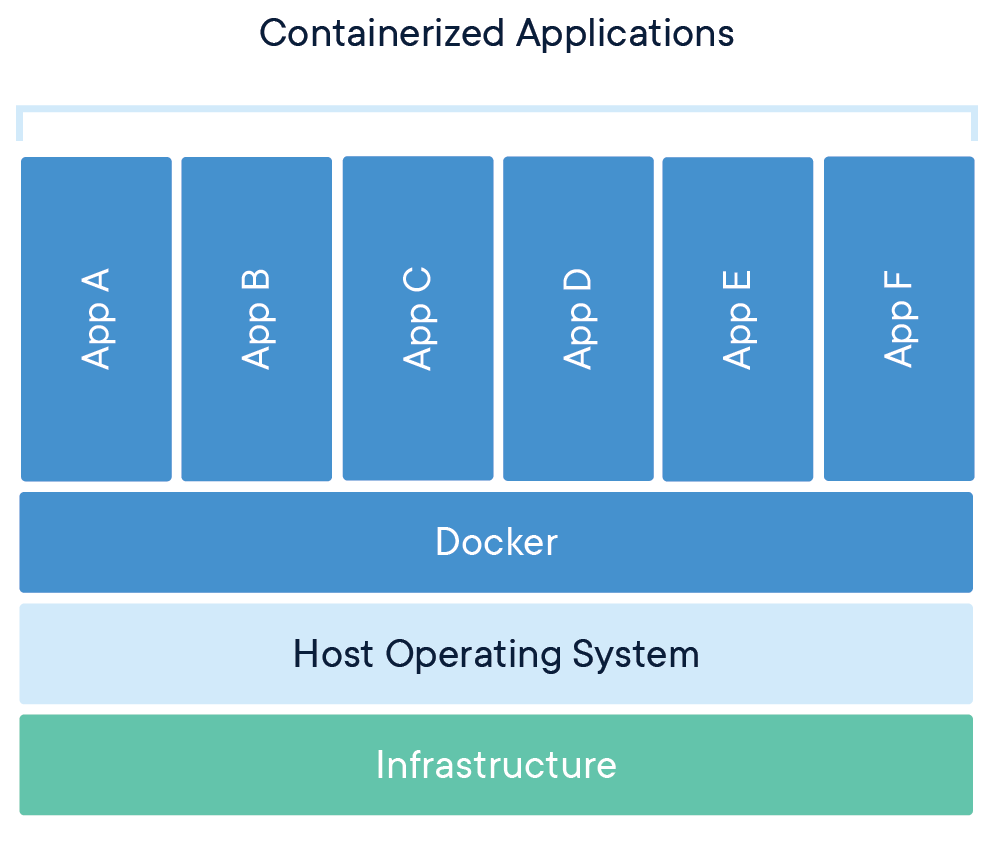
\includegraphics[width=0.45\textwidth]{img/docker-layers}
		\hspace{5mm}
		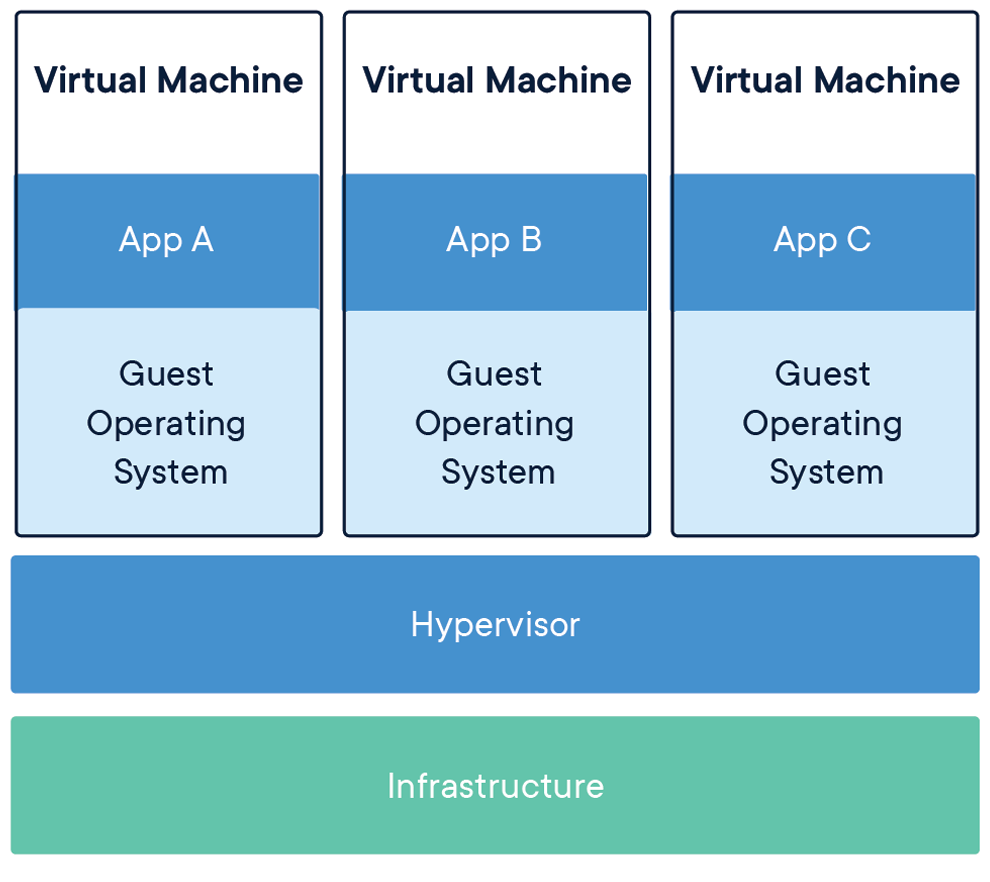
\includegraphics[width=0.45\textwidth]{img/vm-layers}
	\end{center}
	\caption{Docker containers vs VMs \cite{docker-c}.}
	\label{fig:docker-vms}
\end{figure}

\subsection{Docker image}
Jest to plik złożony najczęściej z kilku warstw \cite{docker-doc}. 
Najczęściej wszystkie warstwy oprócz wierchniej są \emph{read-only}, stanowią narzędzia wykorzystywane przez docelową wiechnią aplikację \emph{(np. java sdk)}.
Najwyższa warstwa budowana jest przy pomocy pliku z instrukcją - \emph{\textbf{Dockerfile}}, gdzie dokładamy naszą aplikację.
Przygotowany w ten sposób image jest gotowy do uruchomienia jako kontener. Dużym udogodnieniem dla użytkownika jest globalne publiczne repozytorium docker images - \emph{\textbf{hub.docker.com}}.


\section{Kubernetes}
W zarządzaniu większą ilością produktów AWS stanowiących naszą platformę pomoże nam opisany wcześniej CloudFormation \emph{(\ref{cloudFormation})}. 
W przypadku zarządzania skonteneryzowanymi aplikacjami posłużymy się wiodących standardem w tej dziedzinie - Kubernetes.
Projekt jest rezultatem ponad 10-cio letniego doświadczenia Google w tej dziedzinie opublikowanym na zasadach open-source w 2014 roku \cite{k8s-what}.
Rozwiązanie zyskało na nowych pomysłach społeczności i adaptacji przez wszystkich wiodących dostawców usług chmurowych.
Istnieje również możliwość zastosowania Kubernetes we własnej serwerowni, 
co oznacza duży krok w kierunku jednolitego środowiska niezależnie od sposobu hostowania systemu naszej aplikacji.
Całą strukturę kontenerów jak również i wszystkie inne potrzebne zasoby definiujemy w plikach tekstowych {\em yaml} lub {\em json}.

\subsection{Podstawowe funkcje Kubernetes}

\begin{itemize}
    \item
    \textbf{Service discovery \& load balancing}\\
    Funkcjonalności Kubernetes realizują skonteneryzowane aplikacje systemowe niewidoczne dla użytkownika na porządku dziennym.
    Wśród nich znajdziemy grupę odpowiedzialną za wewnątrz systemowy DNS. Ruch rozkładany jest na ukryte za serwisową domeną instancje aplikacji. 
    
    \item
    \textbf{Storage orchestration}\\
    Automatyczne utworzenie zadanego zasobu pamięci na podstawie definicji tekstowej i dołączenie jej pod wskazany kontener.

    \item
    \textbf{Automatic bin packing}\\
    Mając do dyspozycji zestaw nodów (hostów), na których umożliwiamy stawianie kontenerów, Kubernetes sam podejmuje decyzje na temat wdrożenia.
    Dzięki temu nie musimy się martwić o przeciążenie pojedynczego noda.
    Poprzez definicje wymagań \emph{(CPU, RAM)} danego kontenera możemy natomiast dostarczyć wskazówki. 

    \item
    \textbf{Autoscaling, Self-healing, Automated rollouts and rollbacks}\\
    Za pomocą plików tekstowych definiujemy oczekiwaną liczbę instancji naszej aplikacji i jej zasady skalowania horyzontalnego \emph{(wpływ CPU, RAM)}.
    Ponadto możemy określić sygnały \emph{(np. zapytanie http)} w oparciu o które Kubernetes może weryfikować zdolność do pracy danej instancji, a następnie podjąć próby jej restartu.
    W przypadku utracenia całego noda (hosta) utracone tam kontenery zostaną przerzucone na resztę nodów do czasu startu nowego.
    Domyślnie update kontenera \emph{(np. do nowej wersji docker image)} polega wpierw na uruchomieniu jego nowej wersji, a dopiero potem przepięciu ruchu i zabiciu starej.
    Jeśli nowy kontener nie spełni wymagań żywotności, zostanie on wycofany. Taki proces zapewnia 100\% dostępności aplikacji \cite{k8s-what}.
\end{itemize} 

\chapter{Implementacja}
\label{cha:implementation}

\section{Architektura rozwiązania}

\begin{figure}[!ht]
	\begin{center}
		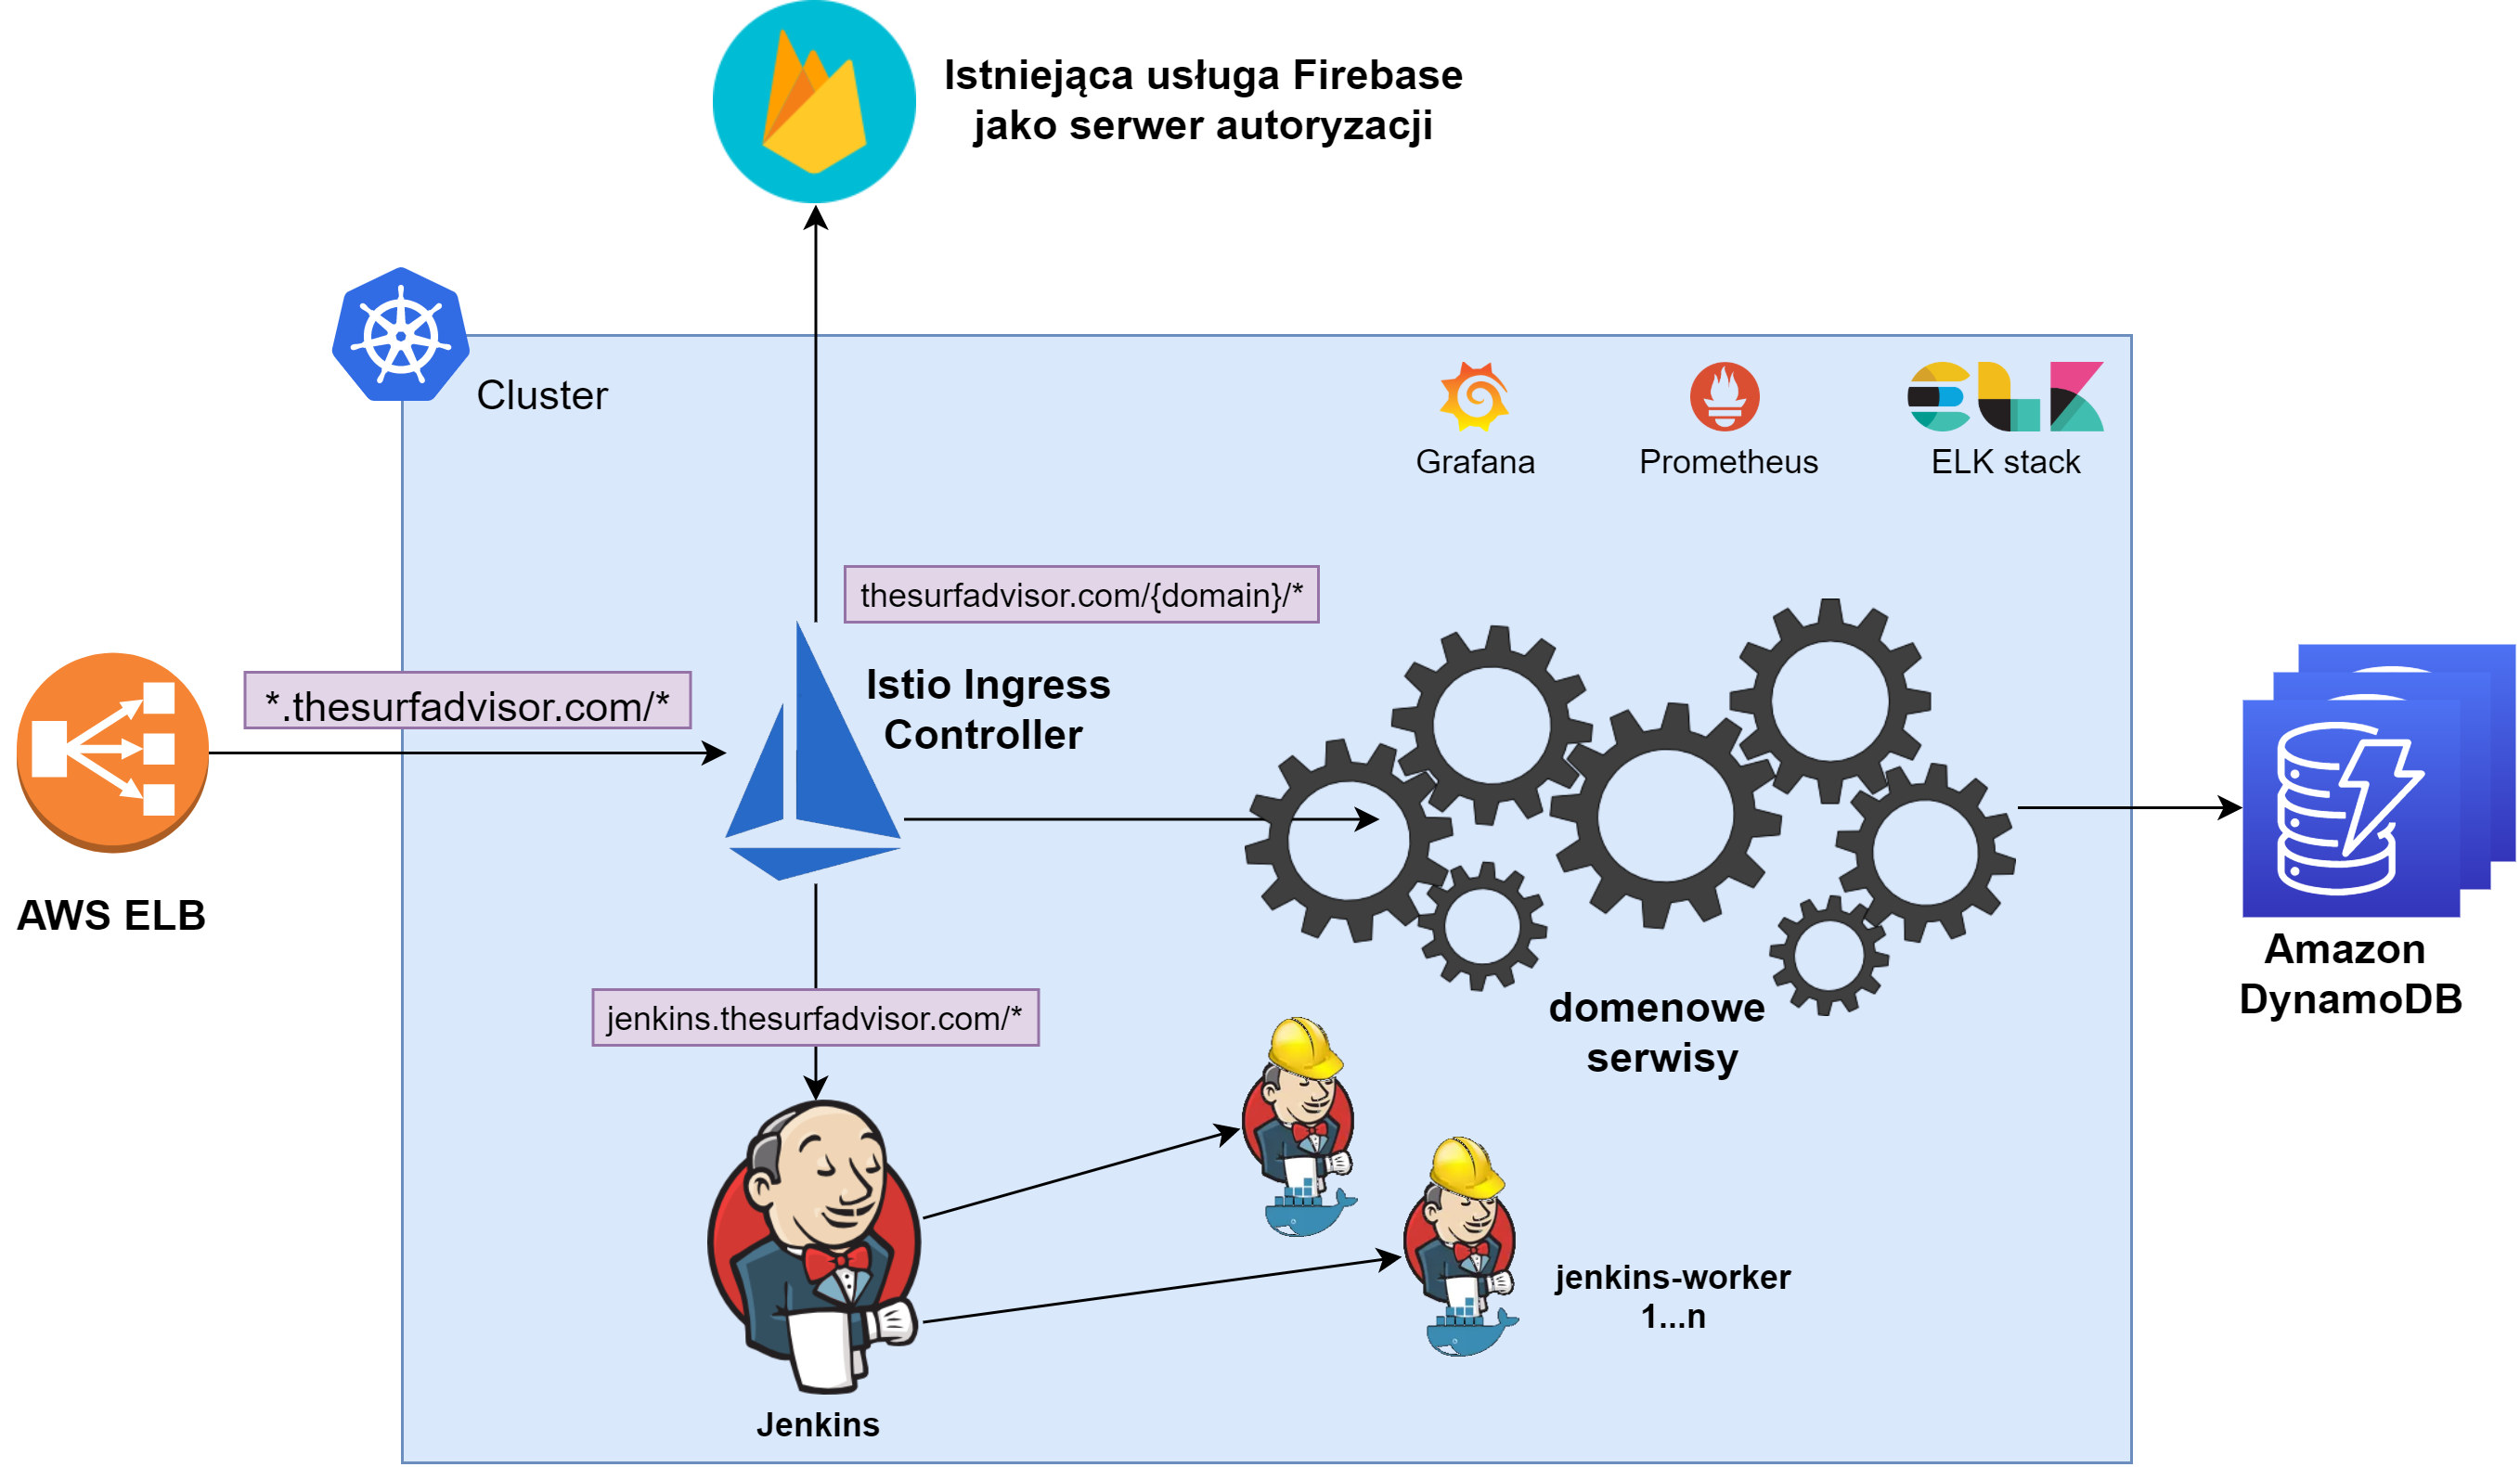
\includegraphics[width=1\textwidth]{img/surf-cluster}
	\end{center}
	\caption{Cluster nowych usług SurfAdvisor}
\end{figure}

\cw{Cluster} nowych usług SurfAdvisor w spoczynku składa się z: 

\begin{itemize}
    \item
    1 x master \cw{Node} - EC2 \textbf{m3.medium} \emph{(1 vCPU \& 3.75 GiB RAM)}

    \item
    2 x worker \cw{Node} - EC2 \textbf{t3.medium} \emph{(2 vCPU \& 4 GiB RAM)}
\end{itemize} 

W przypadku zwiększenia natężenia ruchu liczba \cw{Node}'ów jest skalowana by sprostać wymaganiom.
Pod globalnie dostępną domeną \textbf{thesurfadvisor.com} kryje się \emph{Load Balancer} utrzymywany przez AWS.
Stanowi on jedyny punkt dostępu, cały ruch jest następnie obsługiwany przez Istio \emph{Ingress Controller}.
Autoryzacja zintegrowana jest z istniejącym systemem Firebase. Każdy domenowy serwis uderza do własnej bazy danych DynamoDB.

Jako administrator możemy się dostać do subdomen takich jak:

\begin{itemize}
    \item
    \emph{\textbf{jenkins}.thesurfadvisor.com}\\ 
    Jenkins \emph{WEB UI} pracującego wewnątrz \cw{Cluster}'a

    \item
    \emph{\textbf{grafana}.thesurfadvisor.com}\\
    Grafana \emph{WEB UI} śledząca metryki stanu technicznego

    \item
    \emph{\textbf{kibana}.thesurfadvisor.com}\\
    Kibana \emph{WEB UI} do wygodnego przeszukiwania logów
\end{itemize} 



\section{Aplikacje biznesowe}

\begin{figure}[!ht]
	\begin{center}
		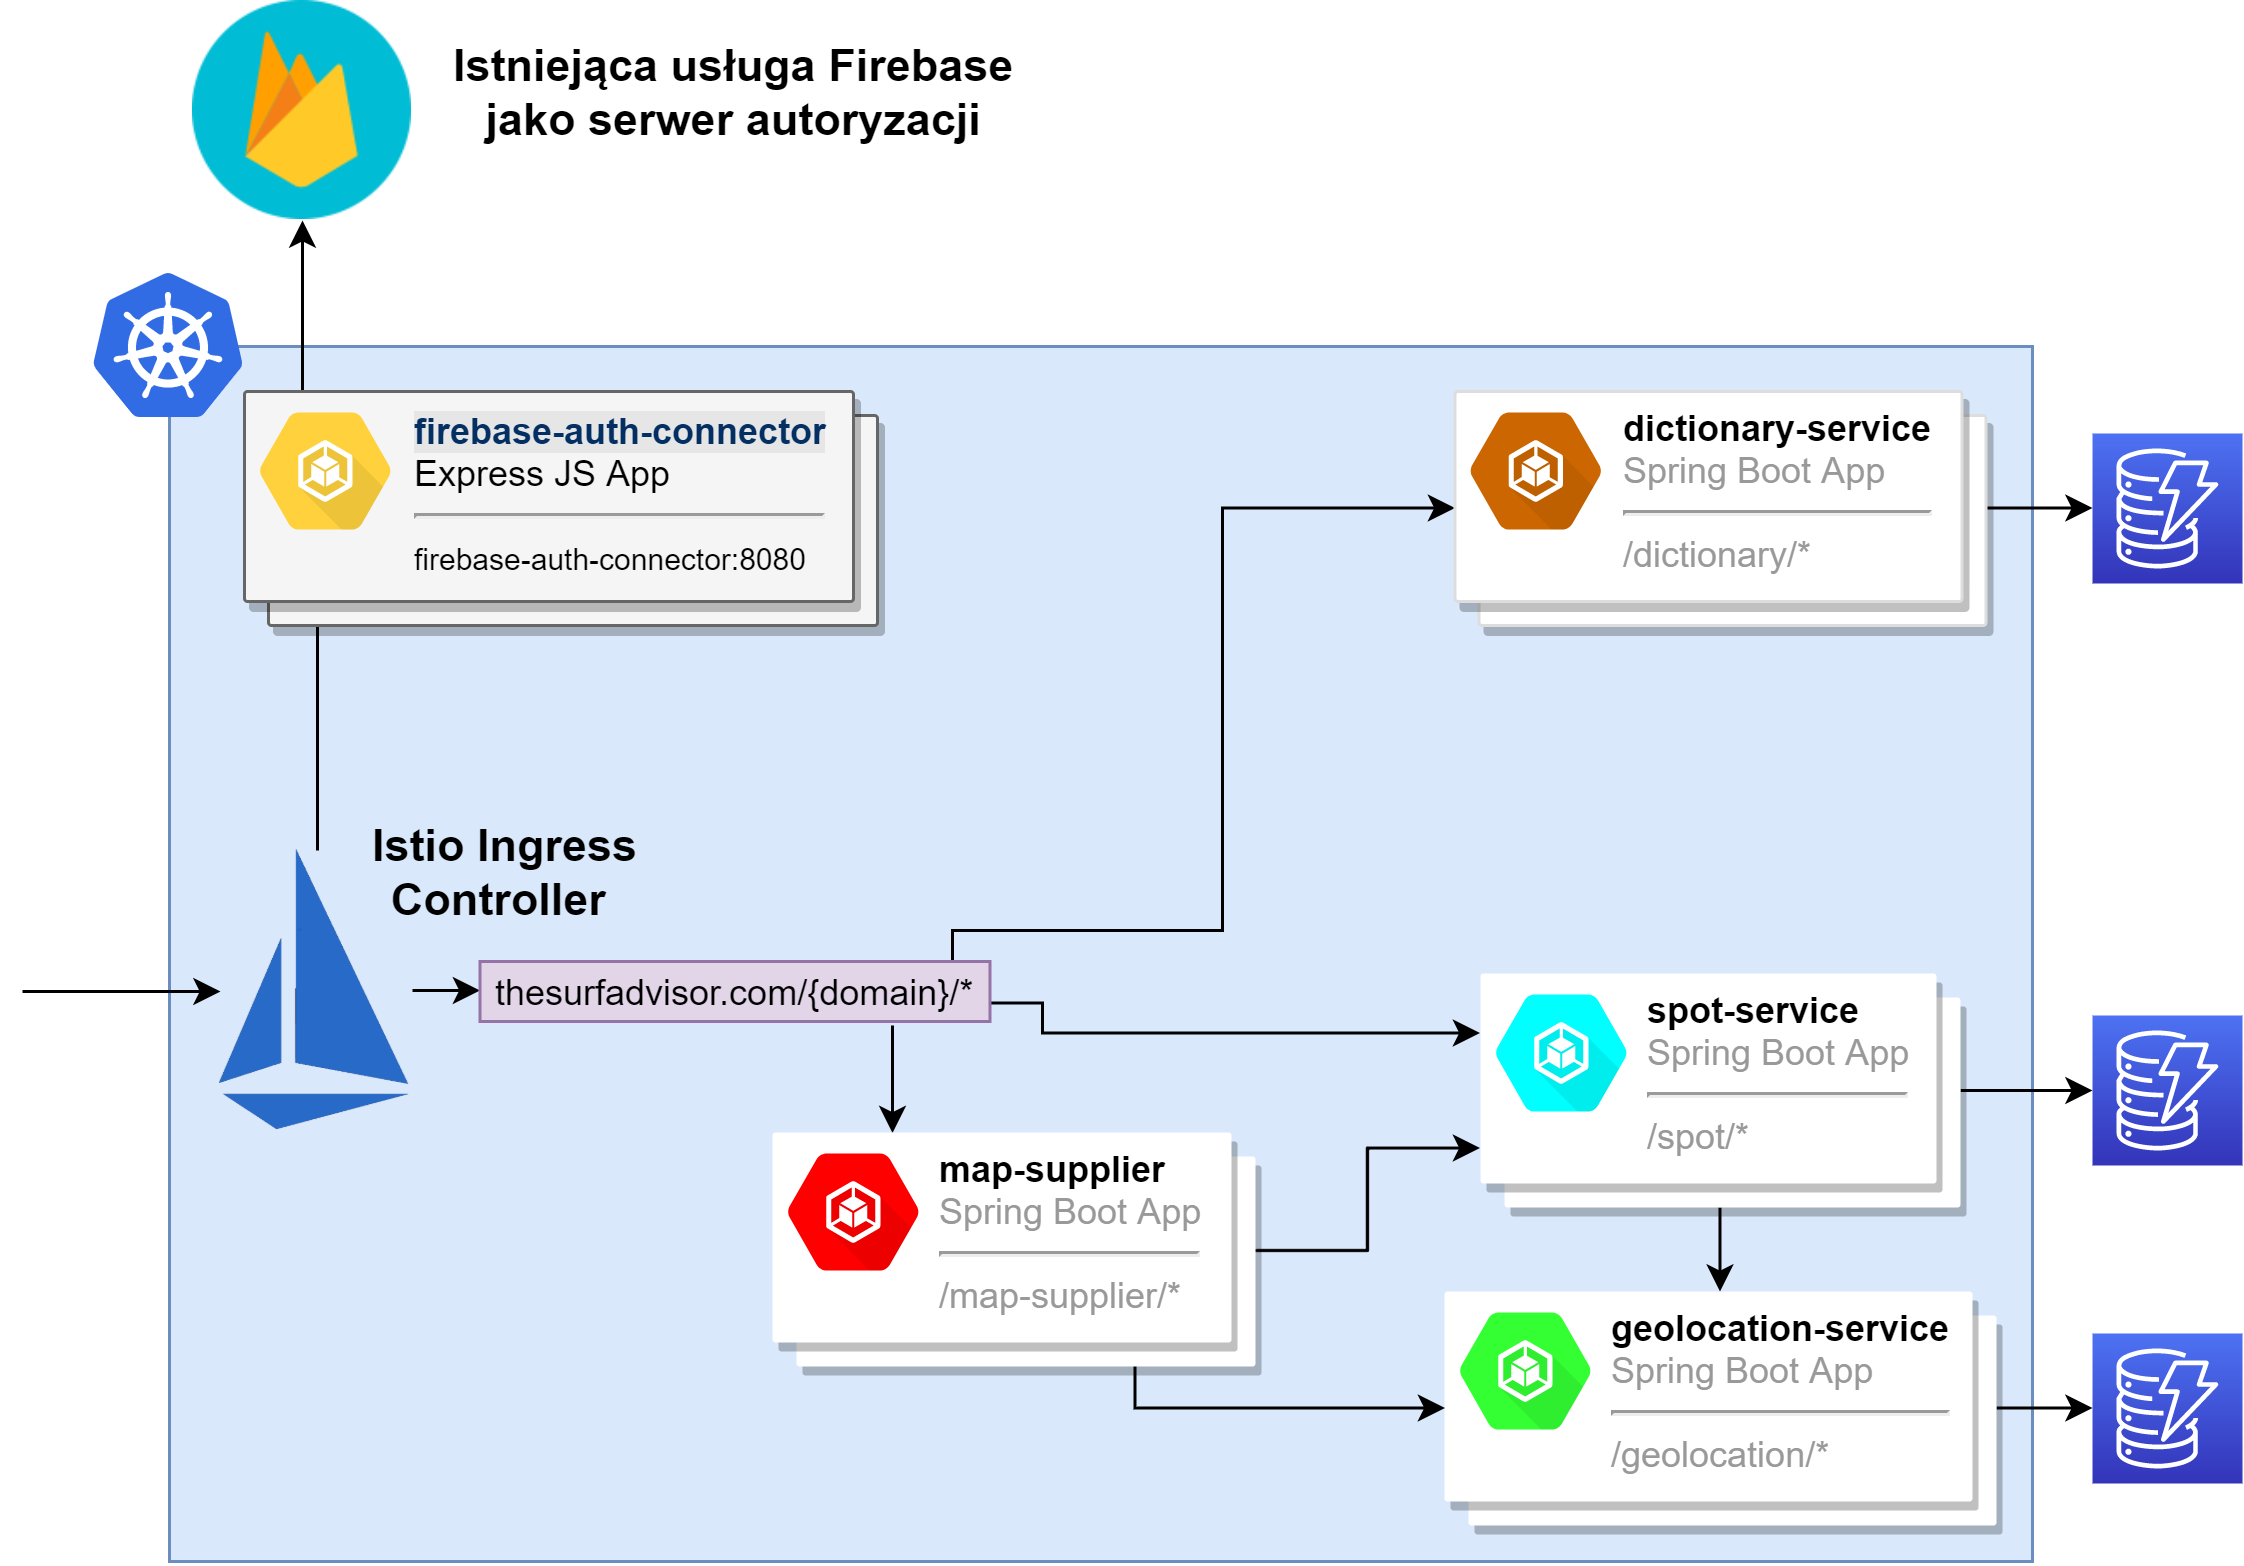
\includegraphics[width=1\textwidth]{img/surf-services}
	\end{center}
    \caption{Zbliżenie na domenowe serwisy SurfAdvisor}
    \label{domain-services}
\end{figure}

\begin{itemize}
    \item
    \textbf{firebase-auth-connector}\\ 
    Warstwa pośrednia pomiędzy Istio \emph{Ingress Controller} a istniejącym serwisem Firebase.
    
    \item
    \textbf{dictionary-service}\\ 
    Repozytorium literałów wyświetlanych w aplikacji mobilnej.

    \item
    \textbf{geolocation-service}\\ 
    Wiedza o położeniu obiektów na kuli ziemskiej.

    \item
    \textbf{spot-service}\\ 
    Atlas spotów - miejsc do uprawiania sportu wodnego.

    \item
    \textbf{map-supplier}\\ 
    Agreguje resztę serwisów związanych z mapą, by wydajniej obsłużyć aplikacje mobilną.
\end{itemize} 




\section{IaC - Infrastructure as Code}

Jest to podejście do zarządzania infrastrukturą \emph{(siecią, wirtualnymi maszynami, kontenerami etc.)} poprzez pliki tekstowe, 
których treść w sposób jednoznaczny definiuje potrzebne zasoby. 
Taką deklaratywną formę konfiguracji bardzo łatwo można śledzić poprzez ten system kontroli wersji co ten używany wokół kodu aplikacji.
IaC jest odpowiedzią na problem różnic pomiędzy środowiskami narastającymi jeszcze bardziej z czasem, jakie powodowały ich manualne imperatywne modyfikacje.
Założeniem IaC jest \textbf{idempotentność} wdrożeń definicji z plików - za każdym razem rezultatem ma być takie samo środowisko \cite{iac-ms}.

W projekcie realizuje tę koncepcję stawiając cały system w czterech krokach. 
Pierwsze trzy stawiają \cw{Cluster} na AWS, są w pełni zautomatyzowane: \emph{CloudFormation}, \emph{Kops} i \emph{Kubernetes}.
Ostatni wdraża domenowe aplikacje, wymaga paru kliknięć w konsoli webowej \emph{Jenkins}'a. 

\subsection{CloudFormation}
\label{iac:cf}

\begin{figure}[!ht]
	\begin{center}
		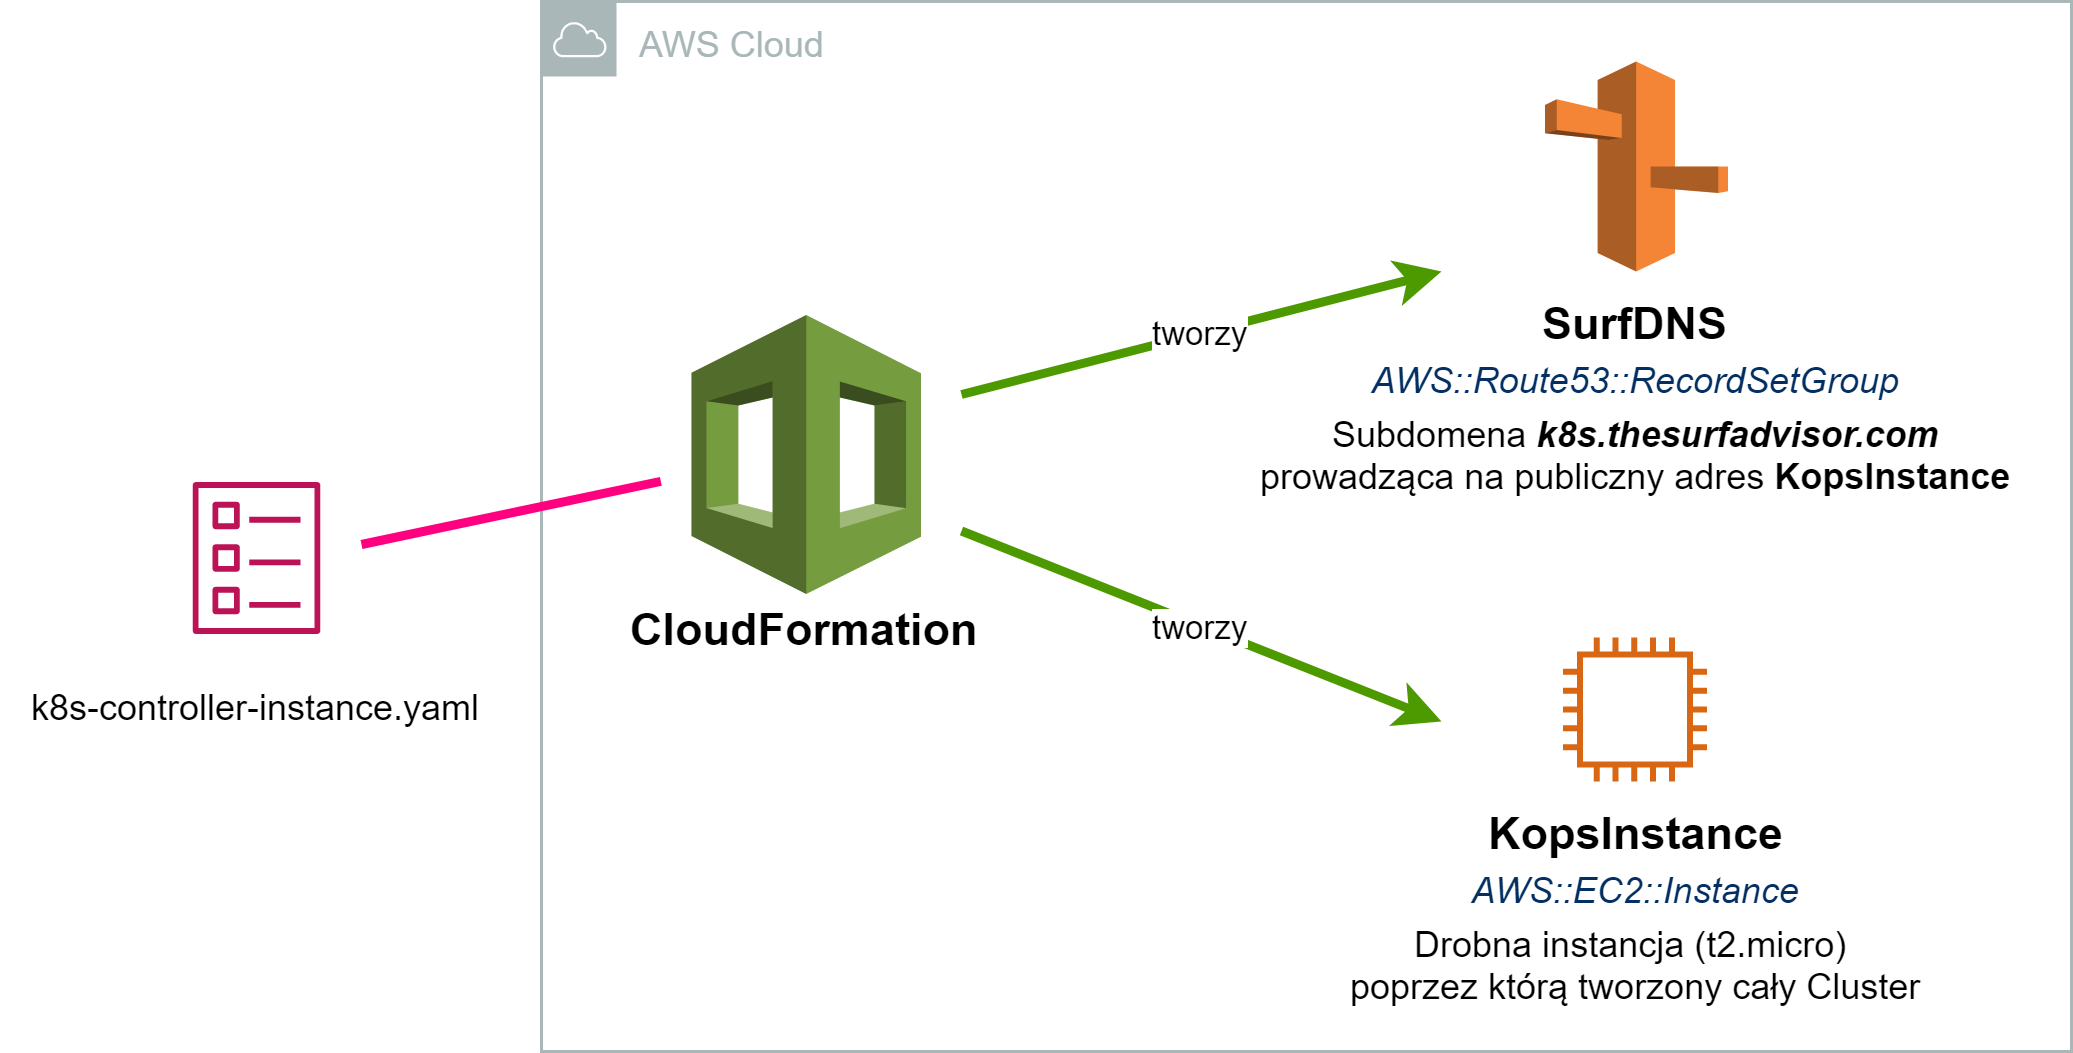
\includegraphics[width=0.9\textwidth]{img/IAC-step1}
	\end{center}
	\caption{Inicjacja Cluter'a SurfAdvisor - 1. CloudFormation}
\end{figure}

Najistotniejszym plikiem CloudFormation w projekcie jest ten inicjujący drobną instancję przeznaczoną do zarządzania docelowym \cw{Cluster}'em.
Plik \cw{k8s-controller-instance.yaml} definiuje głównie: 

\begin{itemize}
    \item
    \textbf{KopsInstance} - drobna instancja linuxa 
    
    \item
    \textbf{SurfDNS} - subdomena oszczędzająca znajomości dokładnego adresu IP \emph{(np. w razie potrzeby ssh)}
\end{itemize} 

Kluczowe znaczenie ma możliwość definicji \emph{\textbf{UserData}} - skryptu \emph{bash} wykonywanego zaraz po starcie instancji. 
Zdefiniowałem w nim polecenia:

\begin{itemize}
    \item
    ściągnięcia dalszych instrukcji \emph{bash} z S3

    \item
    instalacji potrzebnych narzędzi \emph{(kops, kubectl, helm)}
    
    \item
    zbudowania \cw{Cluster}'a poprzez \emph{kops} \emph{(\ref{iac:kops})}

    \item
    wdrożeniu pomocniczych \cw{Service}'ów poprzez \emph{kubectl} \& \emph{helm} \emph{(\ref{iac:kubectl})}
\end{itemize} 

\subsection{Kops}
\label{iac:kops}

\begin{figure}[!ht]
	\begin{center}
		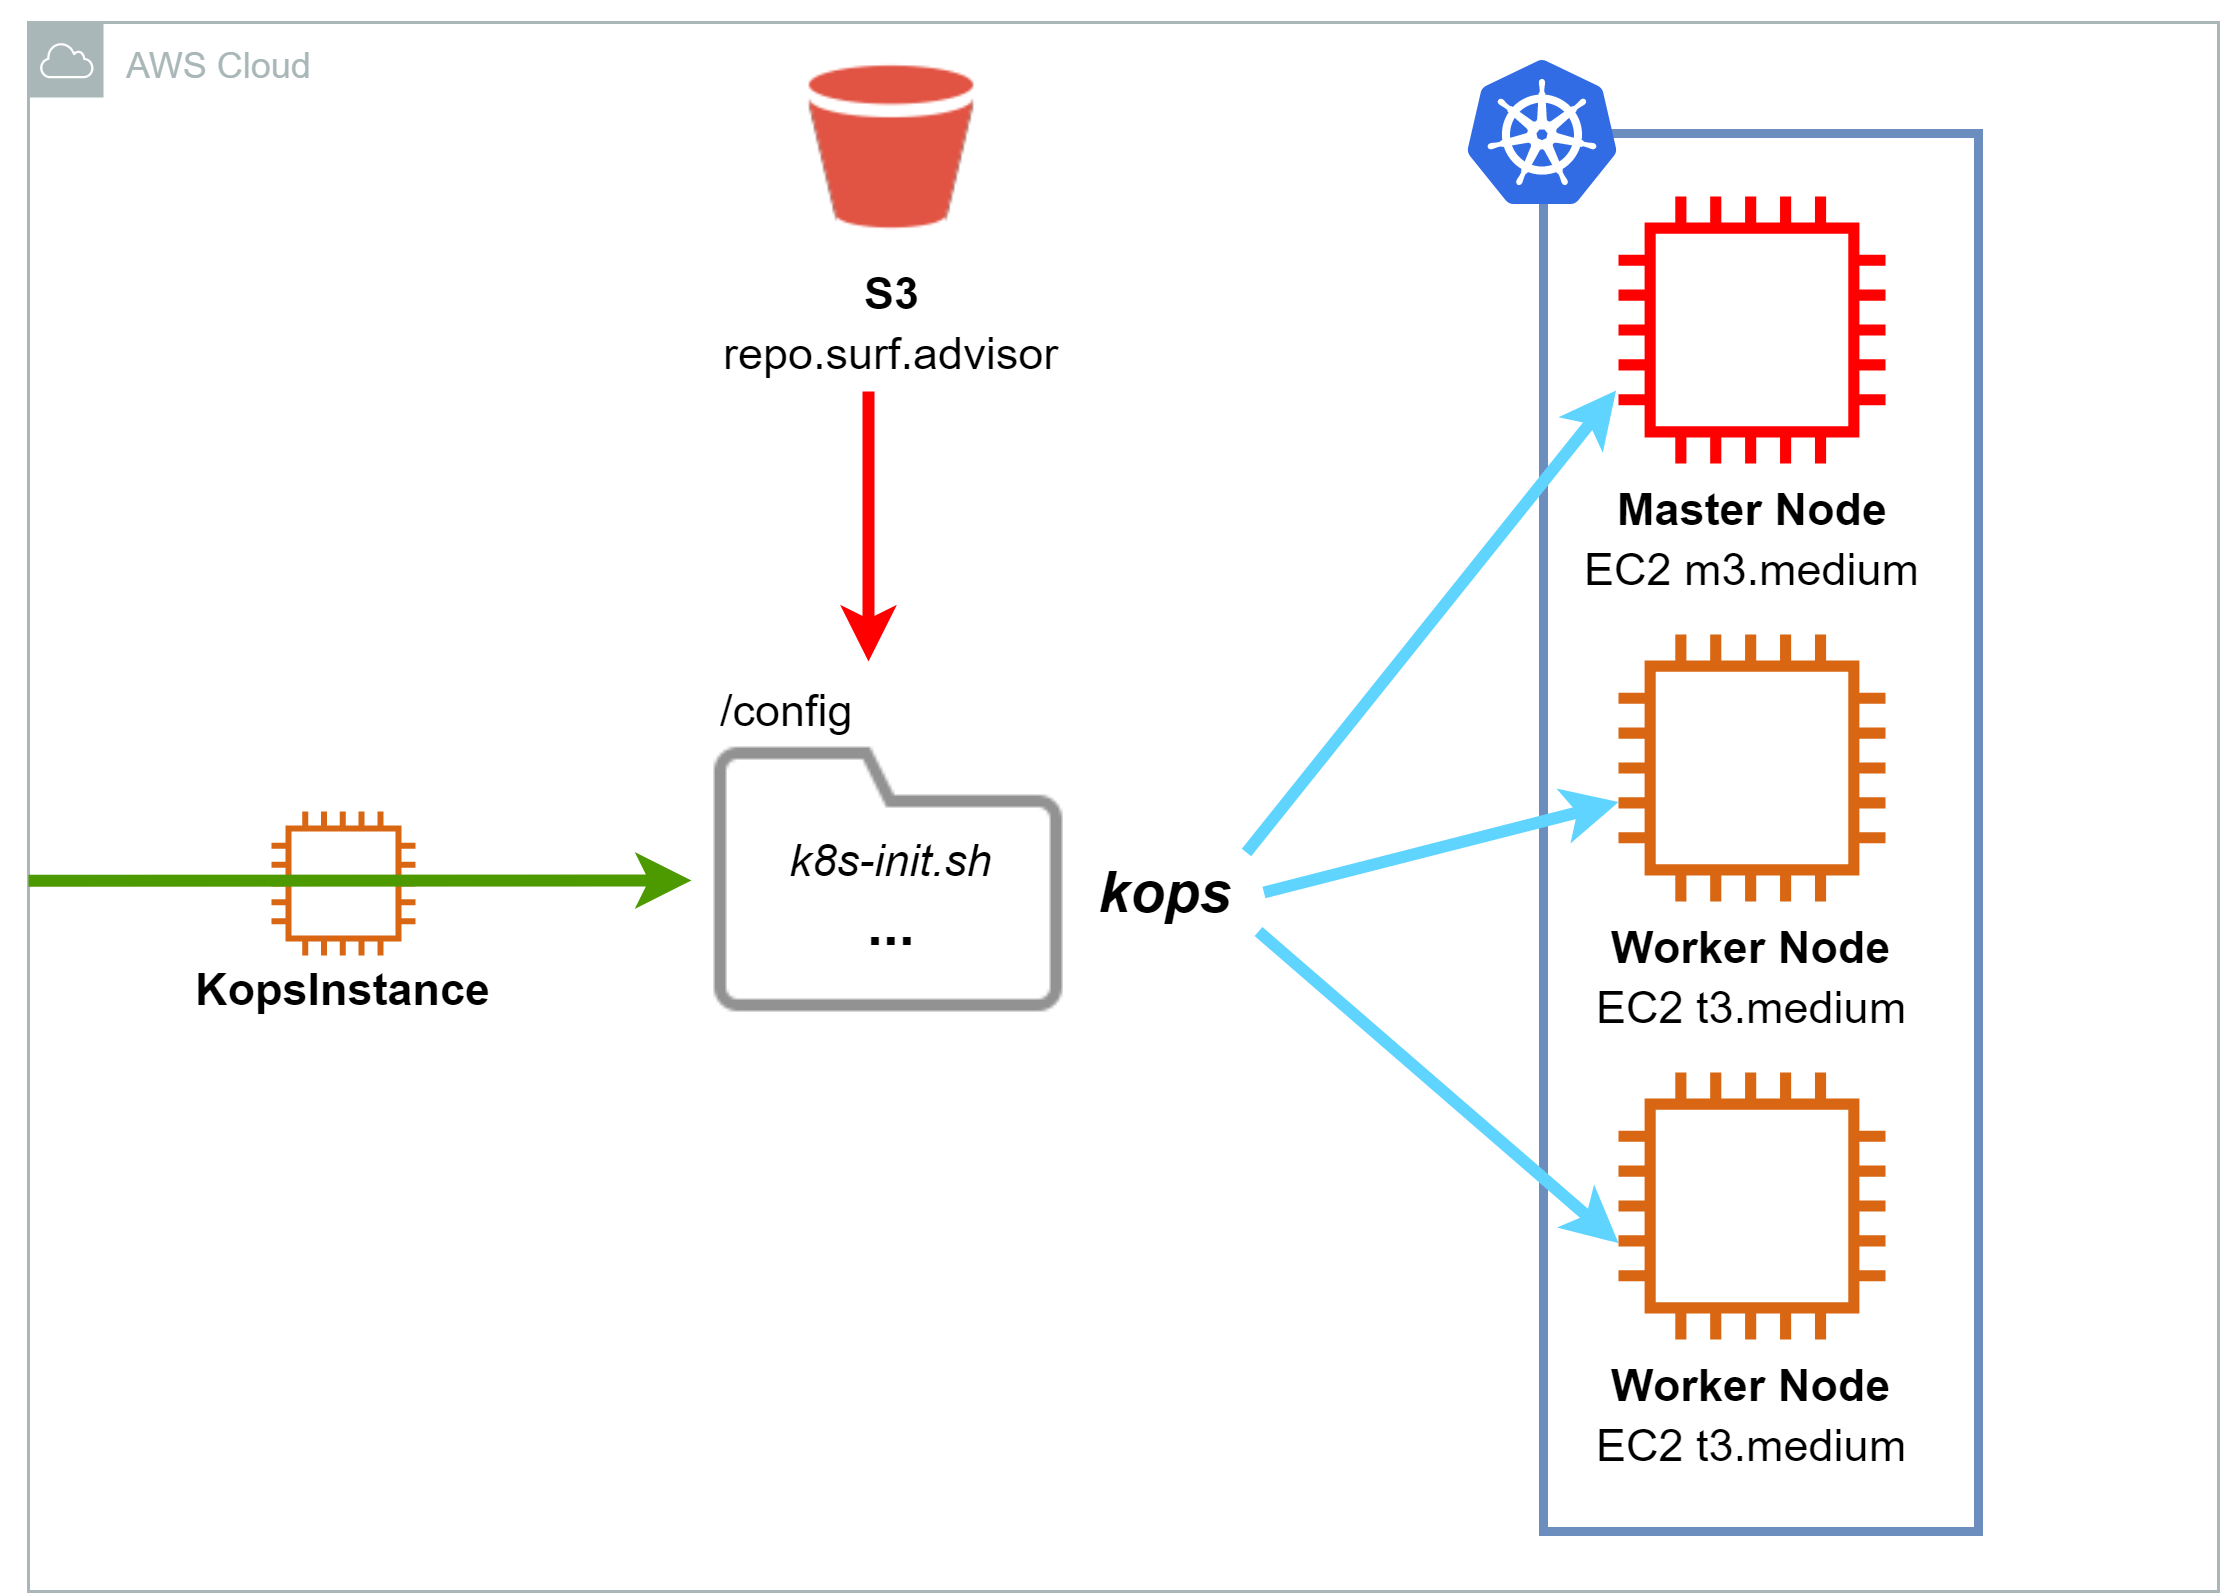
\includegraphics[width=0.95\textwidth]{img/IAC-step2}
	\end{center}
	\caption{Inicjacja Cluter'a SurfAdvisor - 2. Kops}
\end{figure}

\emph{kops} to open-source CLI do budowania \cw{Cluster}'ów Kubernetes na platformie AWS \cite{kops-k8s}.
Stanowi alternatywę dla stosunkowo drogiego na start oficjalnego rozwiązania - EKS \cite{eks-pricing}.

Przy użyciu tego narzędzia dalszy ciąg skryptów, uruchomionych w ramach \emph{UserData} \textbf{KopsInstance} \emph{(\ref{iac:cf})}, buduje \cw{Node}'y składające się na \cw{Cluster}.


\subsection{Kubernetes}
\label{iac:kubectl}

\begin{figure}[!ht]
	\begin{center}
		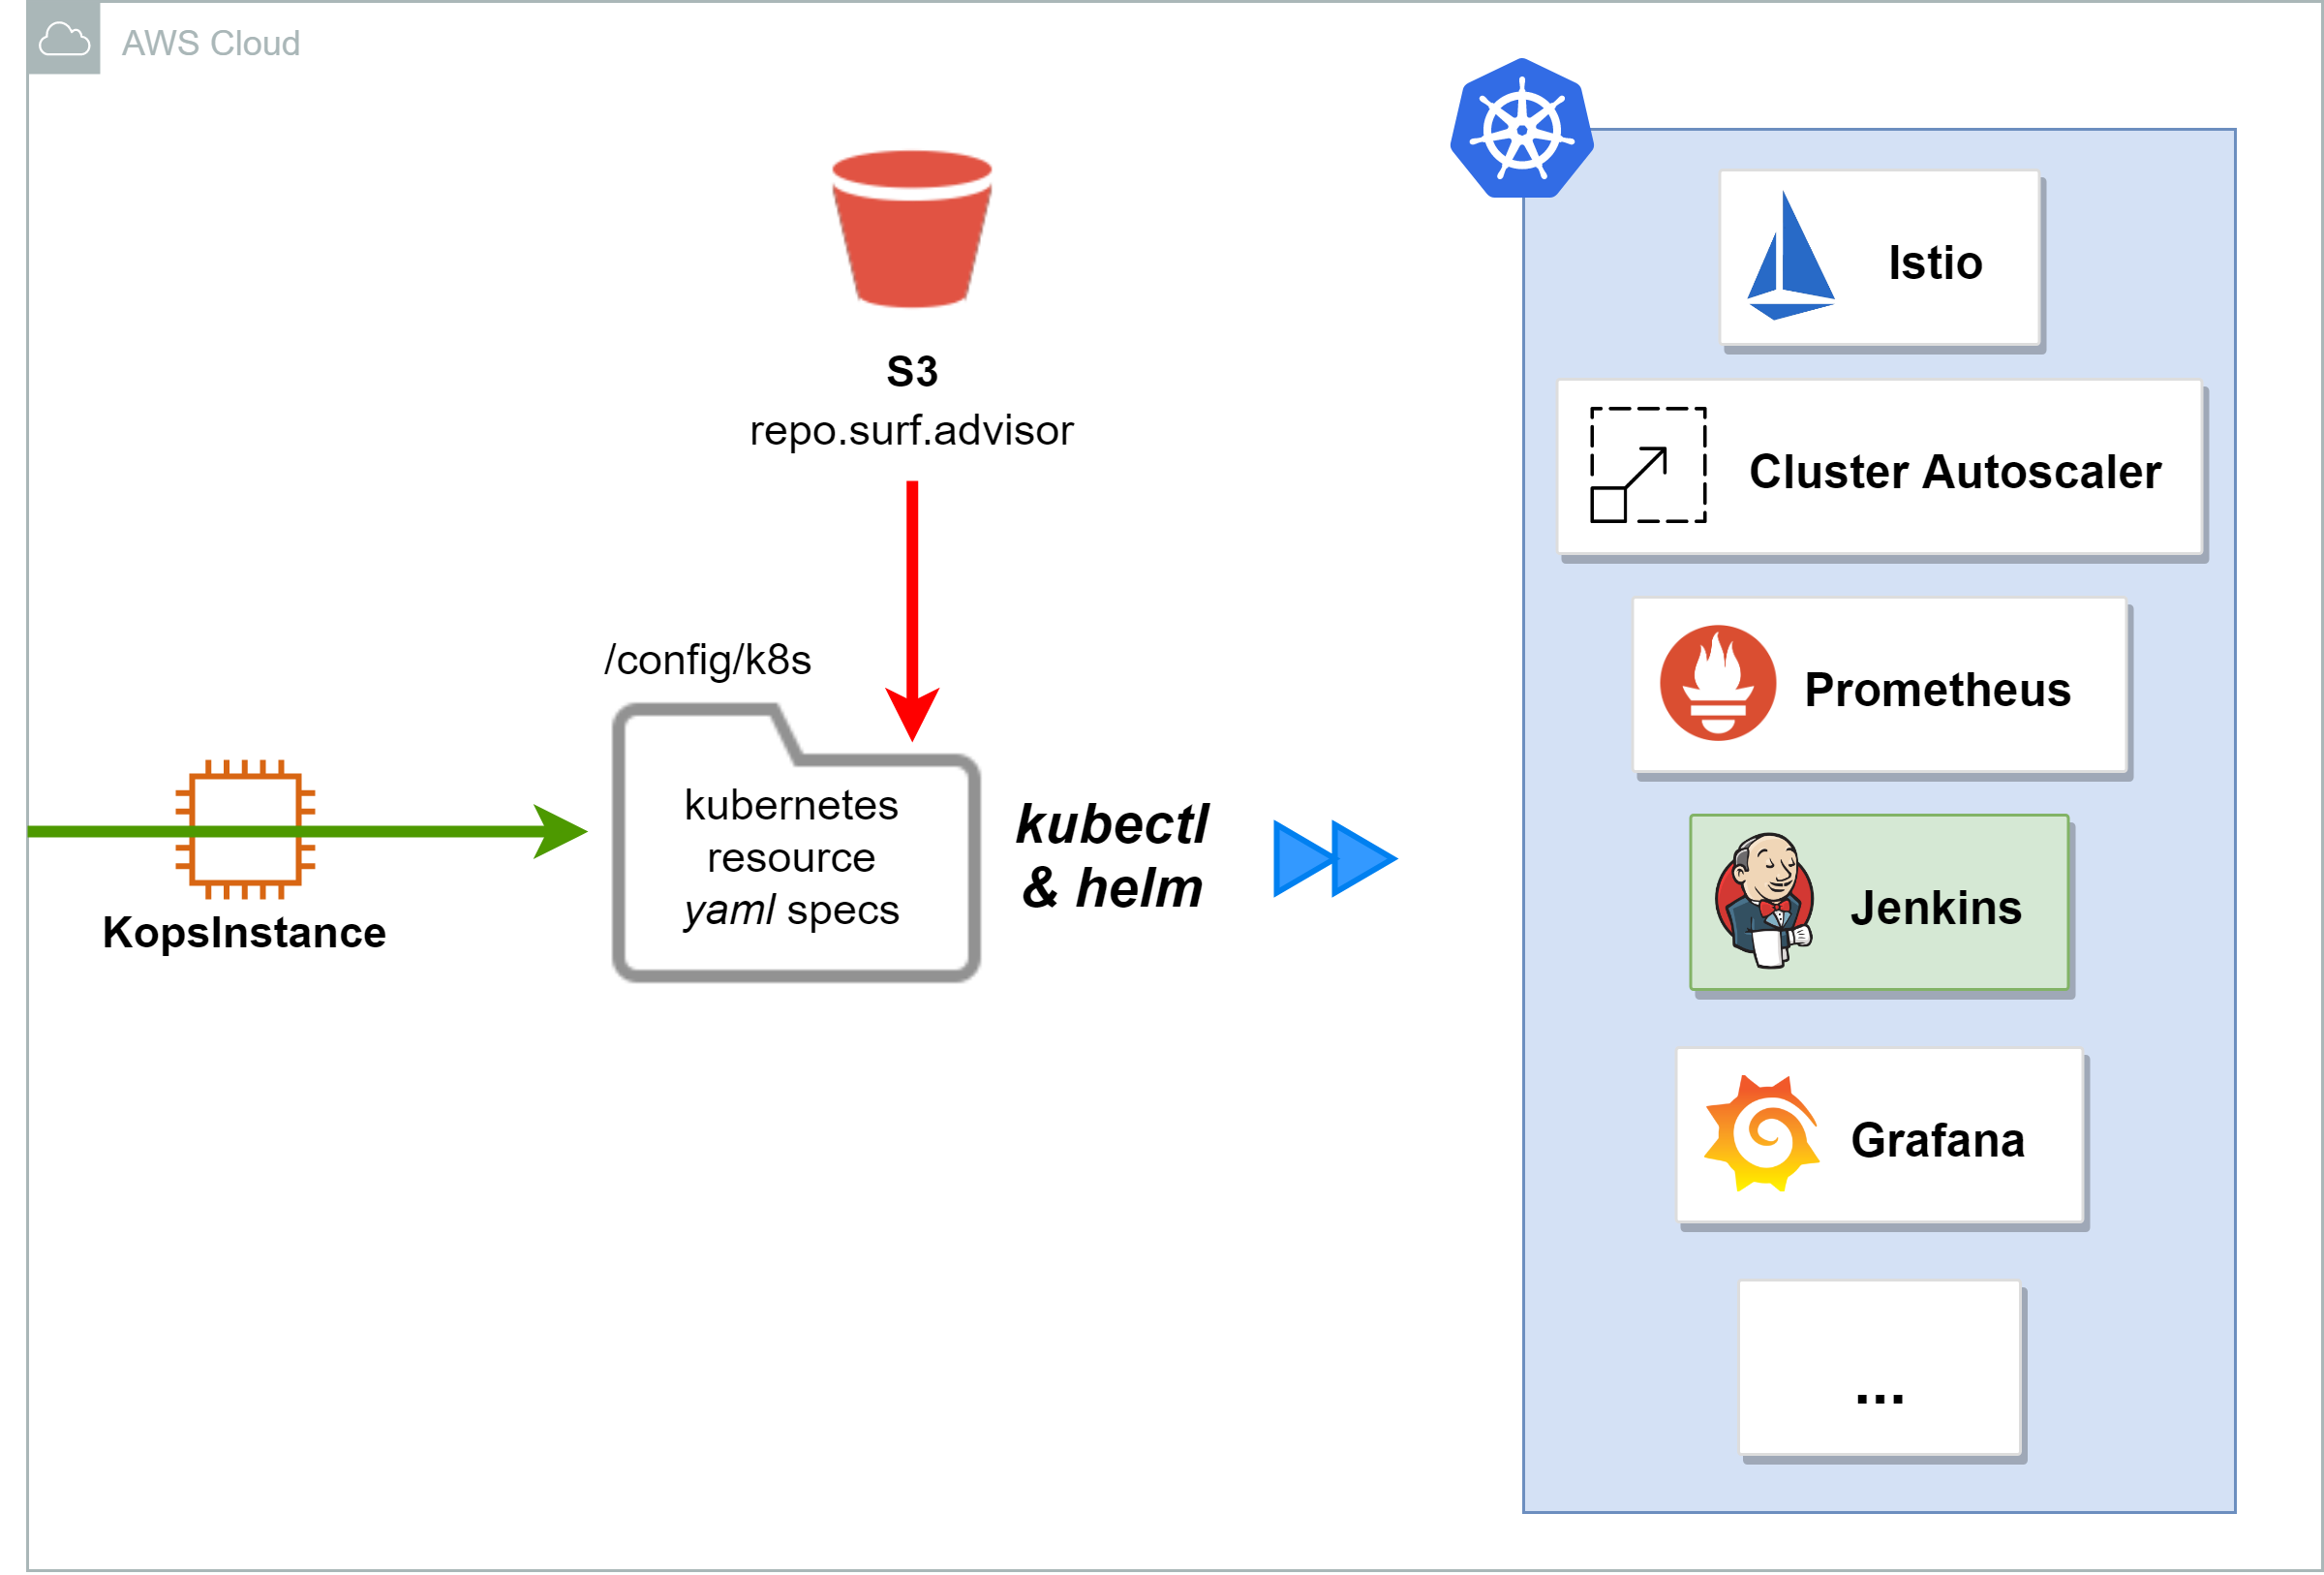
\includegraphics[width=1\textwidth]{img/IAC-step3}
	\end{center}
	\caption{Inicjacja Cluter'a SurfAdvisor - 3. Kubernetes}
\end{figure}

Gdy \emph{kops} skończy już stawiać \cw{Cluster} do akcji wkracza:

\begin{itemize}
    \item
    \emph{\textbf{kubectl}} - oficjalne CLI do operacji na zasobach Kubernetes

    \item
    \emph{\textbf{helm}} - package manager dla Kubernetes
\end{itemize} 

Wdrażane są \cw{Service}'y zaspokajające wymagania bardziej niefunkcjonalne, m.in.:

\begin{itemize}
    \item
    \emph{Jenkins} - który kontynuuje proces inicjacji systemu \emph{[\ref{iac:jenkins}]}

    \item
    \emph{Istio} - sekcja \emph{[\ref{traffic}]}

    \item
    \emph{Prometheus \& Grafana} - monitoring parametrów technicznych \cw{Cluster}'a

    \item
    \emph{Cluster Autoscaler} - rozdział \emph{[\ref{cha:autoscaling}]}
\end{itemize} 


\subsection{Jenkins}
\label{iac:jenkins}

Jenkins jest gotowy do użycia po paru minutach \emph{(wraz ze wszystkimi plugin'ami zdefiniowanymi w pliku konfiguracyjnym)}.
Jedynym manualnym krokiem jaki musimy wykonać jest stworzenie zadania \emph{"Github Organization"}, gdzie podajemy ID naszej organizacji.

\begin{figure}[!ht]
	\begin{center}
		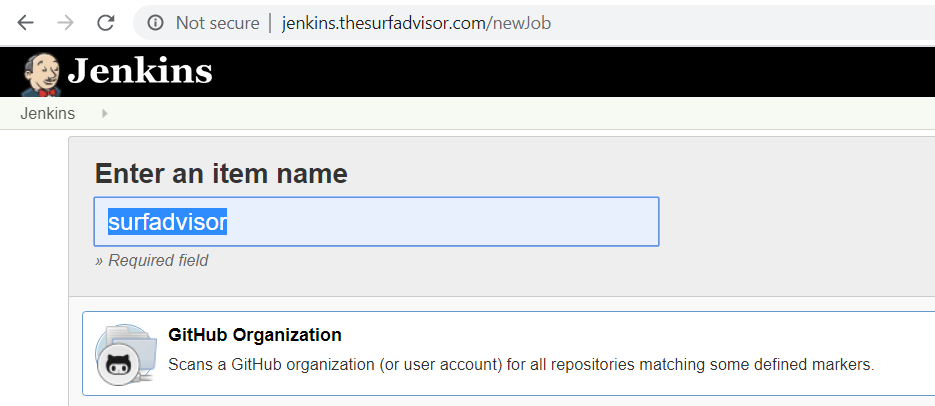
\includegraphics[width=0.8\textwidth]{img/jenkins-new-job}
	\end{center}
	\caption{Jenkins: wdrożenie domenowych serwisów - job "Github Organization"}
\end{figure}

Następnie Jenkins skanuje wszystkie repozytoria widniejące pod daną organizacją i wybiera te zawierące \textbf{\emph{Jenkinsfile}}.
Po chwili będzie dostępna zakładka, na której wylistowane są wszystkie repozytoria spełniające wyżej wymienone kryterium:

\begin{figure}[!ht]
	\begin{center}
		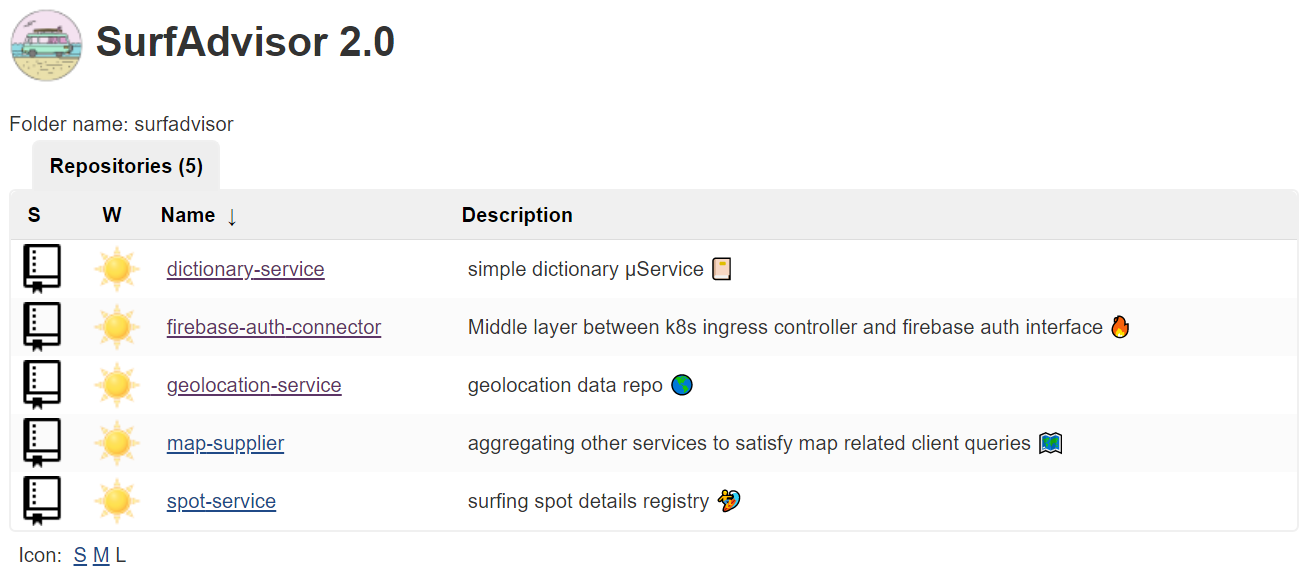
\includegraphics[width=1\textwidth]{img/jenkins-surf-folder}
	\end{center}
	\caption{Jenkins: wdrożenie domenowych serwisów - folder SurfAdvisor}
\end{figure}

Dla każdego z repozytorium Jenkins od razu uruchamia zdefiniowany w \emph{Jenkinsfile} pipeline.
W moim przypadku repozytoria łączy jeszcze obecność dwóch innych plików:
\\\\
\begin{itemize}
    \item
    \emph{\textbf{Dockerfile}} - instrukcja budowy docker image wstawianego potem na DockerHub
    \item
    \emph{\textbf{deploy.yaml}} - deklaracja obiektów Kubernetes: \cw{Service}, \cw{Deployment}, \cw{Pod}, na których stanie dana aplikacja.
    Wdrażane są poprzez \emph{kubectl}.
\end{itemize} 

Poniżej przedstawiony jest wycinek procesowania pipeline dla aplikacji \emph{geolocation-service}.
Dwa końcowe kroki udekorowane są dodatkowo symbolem pliku, na którym polegają.

\begin{figure}[!ht]
	\begin{center}
		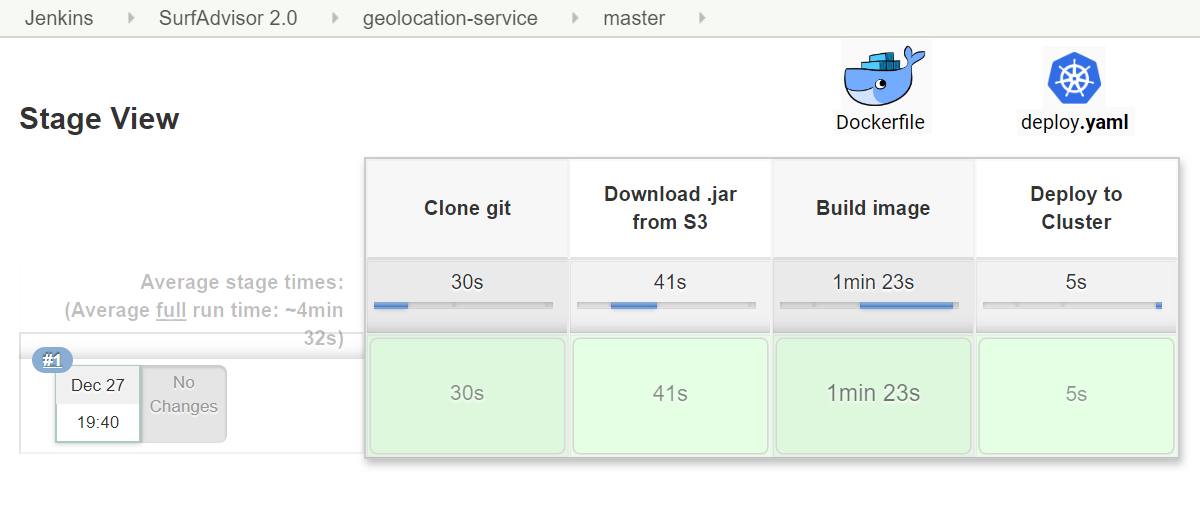
\includegraphics[width=1\textwidth]{img/jenkins-geo-stages}
	\end{center}
	\caption{Jenkins: wdrożenie domenowych serwisów - pipeline}
\end{figure}

\subsection{Usuwanie}

Cały powstały w sposób opisany wyżej \cw{Cluster} wraz ze wszystkimi powiązanymi produktami AWS (\emph{EC2, LoadBalancer, etc.}) usuwa się jedną komendą:

\begin{itemize}
    \item
    \textcolor{blue}{\texttt{kops delete cluster --name \$\{NAME\} --yes}}
\end{itemize} 

Bardzo przydatne na etapie developmentu - usuwamy system kończąc pracę w danym dniu, co przynosi spore oszczędności.

\section{Zarządzanie ruchem i bezpieczeństwo}
\label{traffic}

\begin{figure}[!ht]
    
	\begin{center}
		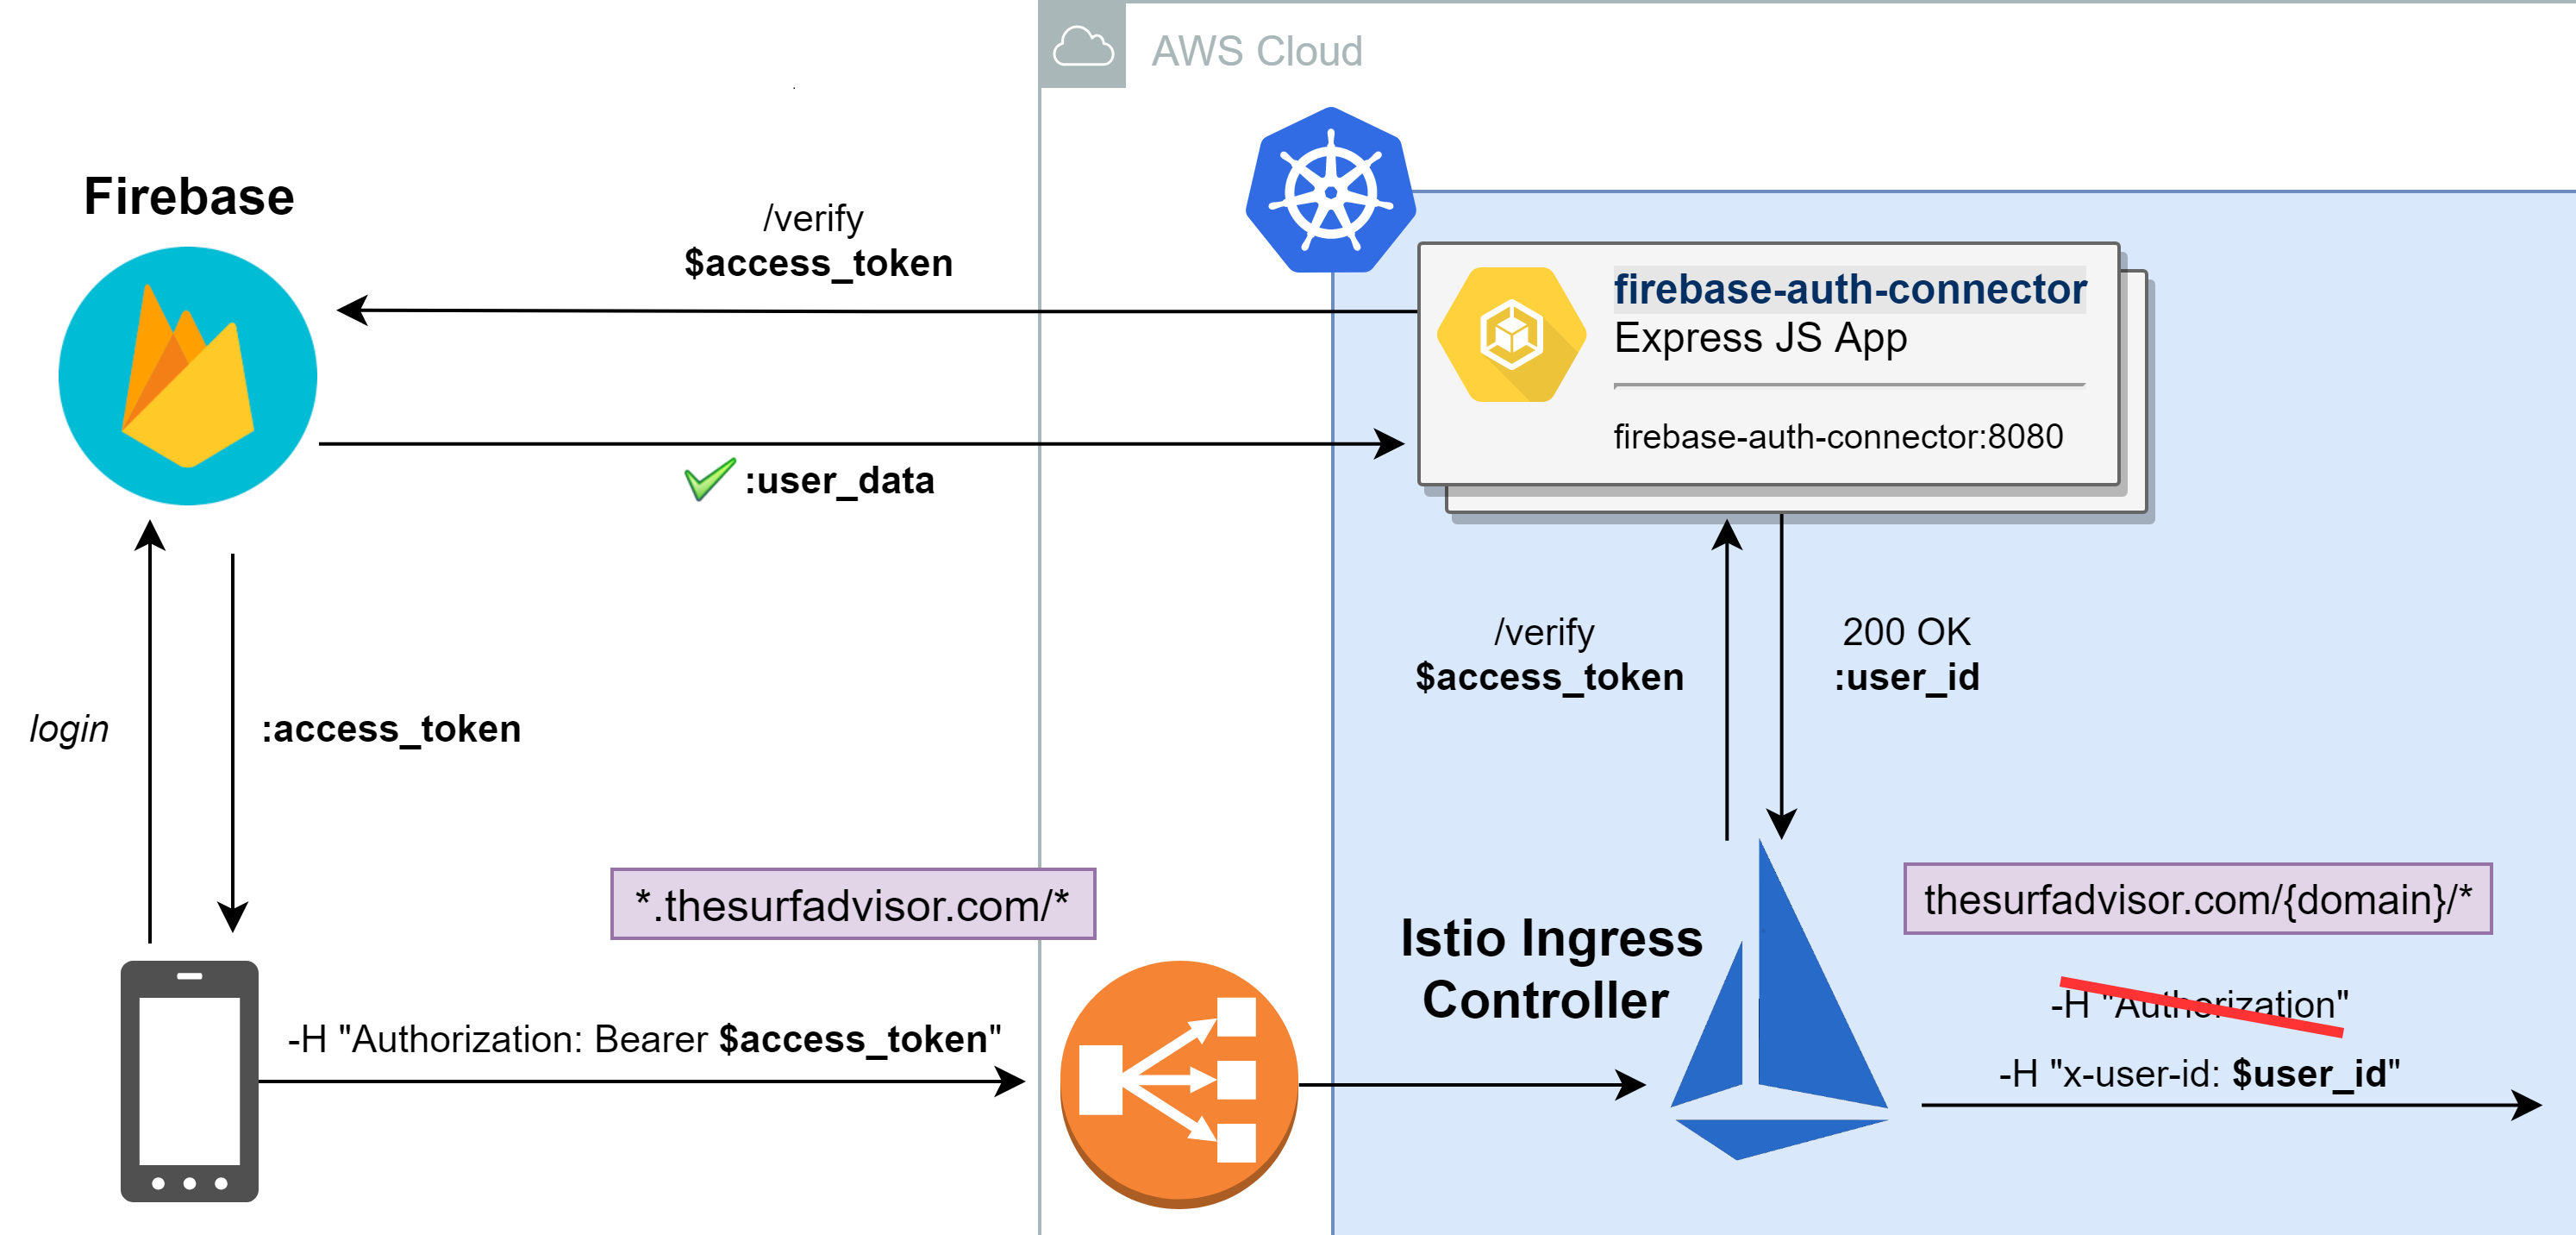
\includegraphics[width=0.93\textwidth]{img/security-flow}
	\end{center}
    \caption{Diagram autentykacji / autoryzacji}
    \label{security-diagram}
\end{figure}

Poprzez ustawienie w Route53 ruch w stronę globalnie dostępnej domeny \emph{\textbf{thesurfadvisor.com}} jest kierowany na Load Balancer, 
który następnie rozrzuca go po \cw{Node}'ach \cw{Cluster}'a.
Na każdym z tych \cw{Node}'ów ruch trafia wpierw do instancji Istio \emph{Ingress Controller}. 
Po pomyślniej autentykacji ruch jest kierowany do odpowiedniego \cw{Service}'u na podstawie ścieżki.
\\\\\\\\
Diagram \ref{security-diagram} ilustruje przebieg autentykacji i autoryzacji:
\begin{enumerate}
    \item
    Proces logowania w aplikacji mobilnej pozostaje bez zmian. Tak jak w starej wersji użytkownik loguje się do Firebase którymś z dostępnych sposobów.

    \item
    Aplikacja mobilna dekoruje zapytania do \emph{thesurfadvisor.com} header'em z tym samym tokenem dostępu, który jest używany do komunikacji z usługami Firebase.

    \item
    Istio \emph{Ingress Controller} deleguje weryfikację nadchodzącego tokena do \cw{Service}'u \textbf{\emph{firebase-auth-connector}}.

    \item
    \emph{firebase-auth-connector} poprzez oficjalne SDK zleca Firebase weryfikację tokena.
    W przypadku sukcesu Firebase zwraca mały zbiór podstawowych danych użytkownika.
    Nasz \cw{Service} zwraca do Istio tylko jego identyfikator, w planach jest dołożenie jeszcze zbioru uprawnień. 

    \item
    Istio usuwa niepotrzebny już header ''Authorization'' i ustawia ''x-user-id'' z identyfikatorem użytkownika.
    W ten sposób dalsze domenowe serwisy są odciążone od implementowania tego aspektu bezpieczeństwa.
\end{enumerate} 



\section{Realizacja wymagań funkcjonalnych}

\subsection{Diagram klas \emph{spot-service} API}

\begin{figure}[H]
	\begin{center}
		\includegraphics[width=1\textwidth]{out/plantuml/spot-api/spot-api.pdf}
	\end{center}
    \caption{Diagram klas \emph{spot-service} API}
    \label{spot-api}
\end{figure}

\subsection{Diagram klas \emph{map-supplier} API}

\begin{figure}[H]
	\begin{center}
		\includegraphics[width=1\textwidth]{out/plantuml/map-supplier-api/map-supplier-api.pdf}
	\end{center}
    \caption{Diagram klas \emph{map-supplier} API}
    \label{ms-api}
\end{figure}


\begin{figure}[H]
	\begin{center}
		\includegraphics[width=0.1\textwidth]{out/plantuml/map-query-flow/map-query-flow-empty.pdf}
	\end{center}
\end{figure}

\subsection{Zasilanie mapy spotów}

\begin{figure}[H]
	\begin{center}
		\includegraphics[width=0.92\textwidth]{out/plantuml/map-query-flow/map-query-flow.pdf}
	\end{center}
\end{figure}

Większość funkcjonalności zaimplementowanych w ramach tego projektu bierze udział podczas zasilania mapy spotów.
Topologia domenowych \cw{Service}'ów pokazana jest na diagramie \ref{domain-services}. 
Poprzez analizę przebiegu zapytania o punkty na mapie poznamy głębiej poszczególne \cw{Service}'y.

\begin{enumerate}
    \item
    \large{\emph{[map-supplier]} - \textbf{GET /rectangle} (query)}\normalsize\\
    nadchodzące od aplikacji mobilnej zapytanie jest typu \cw{RectangleMapQuery} (\ref{ms-api}), zawiera:
    \begin{itemize}
        \item
        \textbf{\emph{rectangle}} - w zamyśle obszar widoczny na mapie

        \item
        \textbf{\emph{objectTypes}} - żądane typy obiektów, aktualnie są to tylko spoty, ale w przyszłości typów może być więcej

        \item
        \textbf{\textcolor{blue}{\emph{spotFilters}}} - filtry dla obiektów typu spot, w przyszłości w zapytaniu mogły by się pojawić filtry dla pozostałych typów

        \item
        \textbf{\emph{referenceLocation}} - punkt na mapie \emph{(w zamyśle położenie użytkownika)}, wobec którego liczone są odległości zwracanych punktów
    \end{itemize} 


    \item
    \large\emph{[map-supplier]} - \textbf{dyskretyzacja obszaru}\normalsize\\
    Wartości szerokości i długości geograficznej jakie mogą nadejść od klienta są praktycznie liniowe.
    Szansa na powtórzenie się obszaru jest bardzo niska. Stąd pojawiła się potrzeba przybliżenia tych wymiarów do najbliższych zdefiniowanych dyskretnych wartości.
    W ten sposób szansa potwórki jest znacznie większa. Oznacza to, że aplikacja częściej będzie mogła skorzystać z \textbf{cache}'a.
    Poniższy wykres przedstawia użytą funkcję dyskretyzacji, która zmiejsza swój stopień wraz z przybliżeniem na mapie.

    \begin{figure}[H]
        \begin{center}
            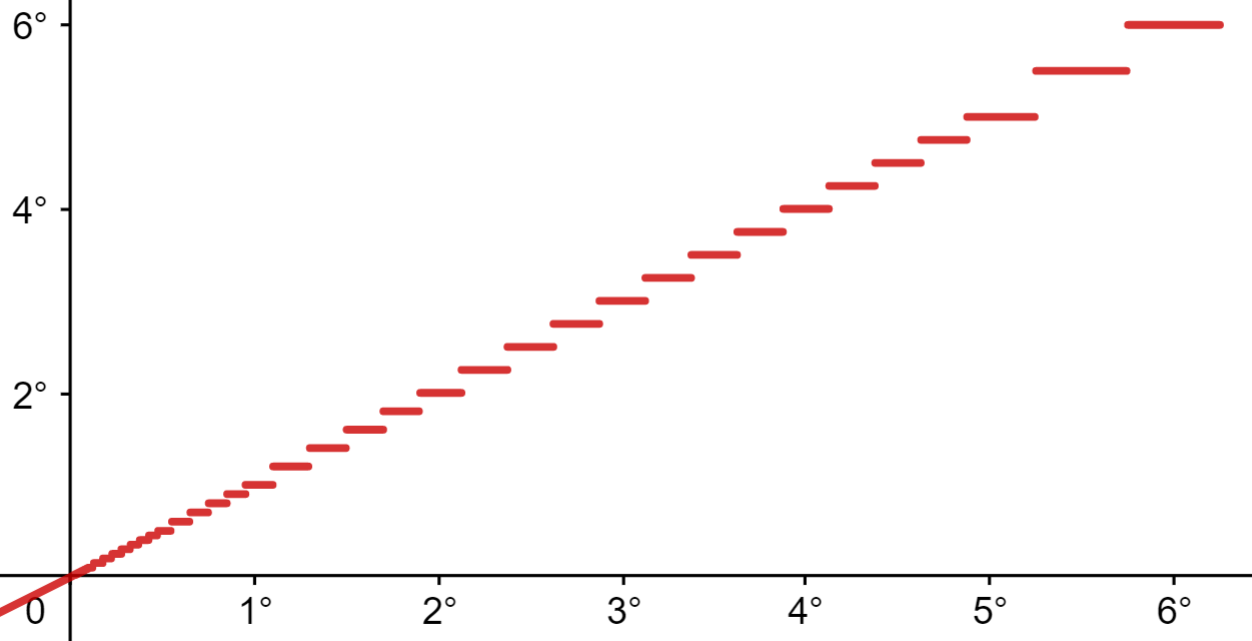
\includegraphics[width=0.5\textwidth]{img/lat-long-discretization}
        \end{center}
        \caption{Funkcja dyskretyzacji kąta}
    \end{figure}

    \item
    \large\emph{[geolocation-service]} - \textbf{selectByGeohash}\normalsize\\
    \emph{Geohash} w dużym skrócie jest funkcją dyskretyzacji powierzchni globu.
    Zamienia długość i szerokość geograficzną na identyfikator wycinka Ziemi, w którym się znajduje.
    W ten sposób poindeksowane są obiekty w tabeli \cw{GEOLOCATION}. Znacznie przyspiesza to zapytania punkty w zadanym obszarze.

    \item
    \large\emph{[geolocation-service]} - \textbf{klasteryzacja}\normalsize\\
    Wykonywana jest po stronie backendu, aby nie obarczać tym zadaniem aplikacji mobilnej. 
    W zależności od stopnia przybliżenia wykorzystywany jest jeden z trzech algorytmów:

    \begin{itemize}
        \item
        \textbf{\emph{Geohash}} - klasteryzacja na podstawie \emph{Geohash}'u

        \item
        \textbf{\emph{DBSCAN}} - algorytm opierający się na gęstości punktów

        \item
        \textbf{\emph{k-means}} - kieruje się średnią odległością dzielącą punkty

    \end{itemize} 
    

    \item
    \large{\emph{[spot-service]} - \textbf{GET /spots/filter-ids} (spotFilters)}\normalsize\\
    \emph{Geolocation-service} zwraca sklasteryzowane identyfikatory obiektów w zadanym obszarze.
    Teraz pora na filtrowanie tego zbioru po zadanych w zapytaniu parametrach.
    To zadanie należy do \emph{spot-service}. Zwraca on zbiór identyfikatorów spełniających kryteria.

    \item
    \large{\emph{[geolocation-service]} - \textbf{GET /geolocations}/\{uid\}}\normalsize\\
    W przypadku gdy grupa identyfikatorów stanowiąca klaster zostanie zredukowana po filtrowaniu do pojedynczego punktu, wypada skorygować jego koordynaty.
    Wołany jest wtedy \emph{geolocation-service} by pozyskać dokładny punkt.

    \item
    \large{\emph{[spot-service]} - \textbf{GET /spots}/\{uid\}}\normalsize\\
    Każdy pojedynczy punkt dekorowany jest skojarzonymi danymi spotu, klastry są pomijane.

    \item
    \large\emph{[map-supplier]} - \textbf{MapSupplierResponse}\normalsize
    \begin{itemize}
        \item
        \textbf{\emph{matchedRectangle}} - użyty obszar po dyskretyzacji

        \item
        \textbf{\emph{points}} - wynikowe obiekty - klastry lub pojedyncze spoty

    \end{itemize} 
    
\end{enumerate}

\pagebreak

\subsection{Aplikacja mobilna}

\begin{figure}[h!]
	\begin{center}
		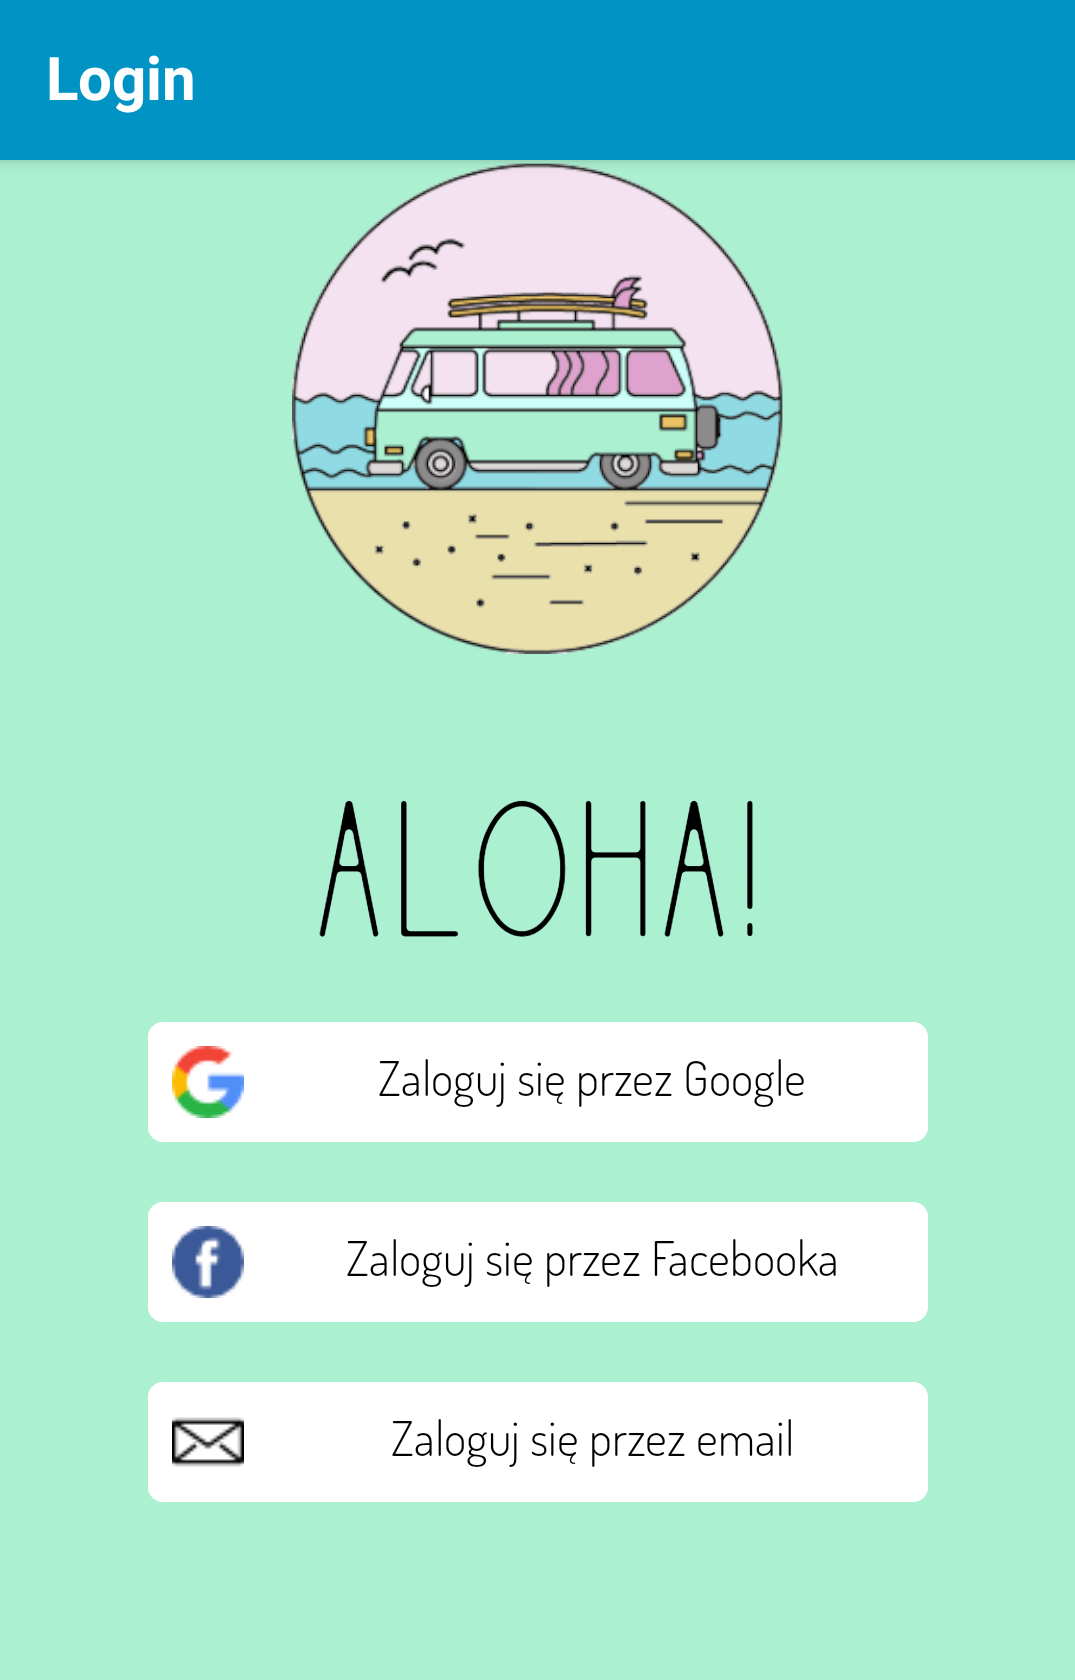
\includegraphics[width=0.45\textwidth]{img/mobile/login}
		\hspace{5mm}
		
\includegraphics[width=0.45\textwidth]{img/mobile/google}
	\end{center}
	\caption{...}
\end{figure}

\begin{figure}[h!]
	\begin{center}
		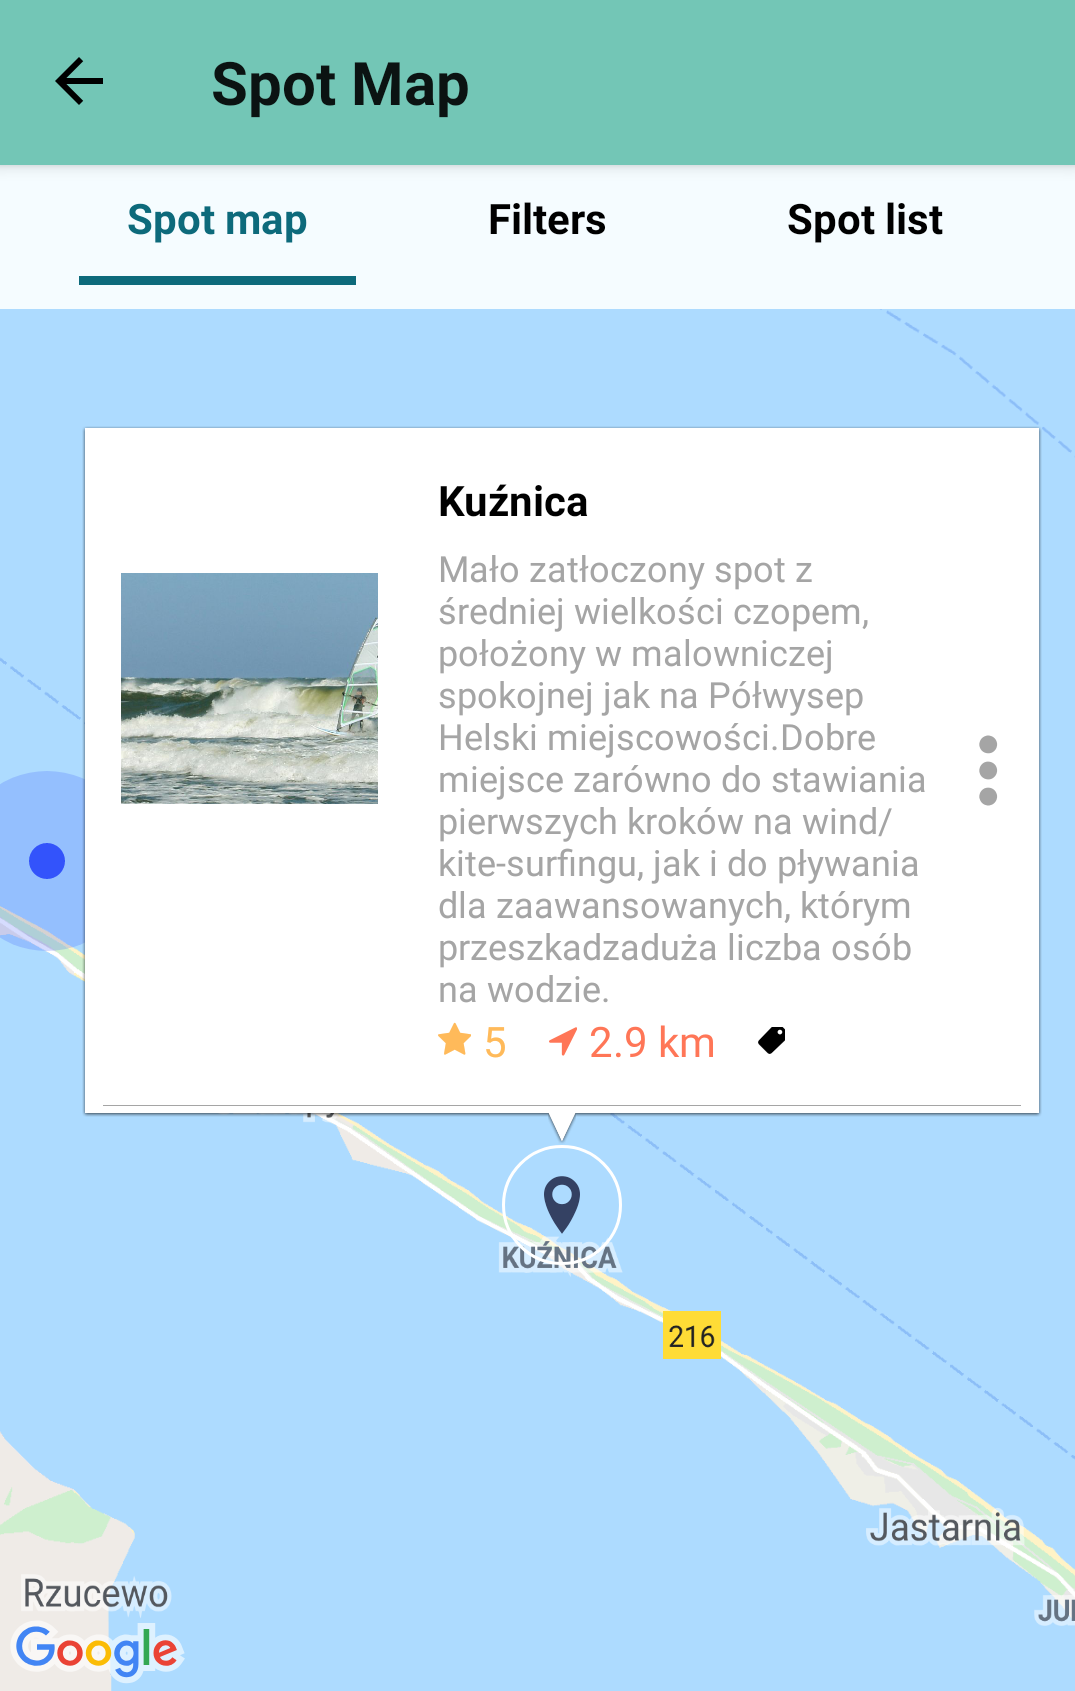
\includegraphics[width=0.45\textwidth]{img/mobile/map}
		\hspace{5mm}
		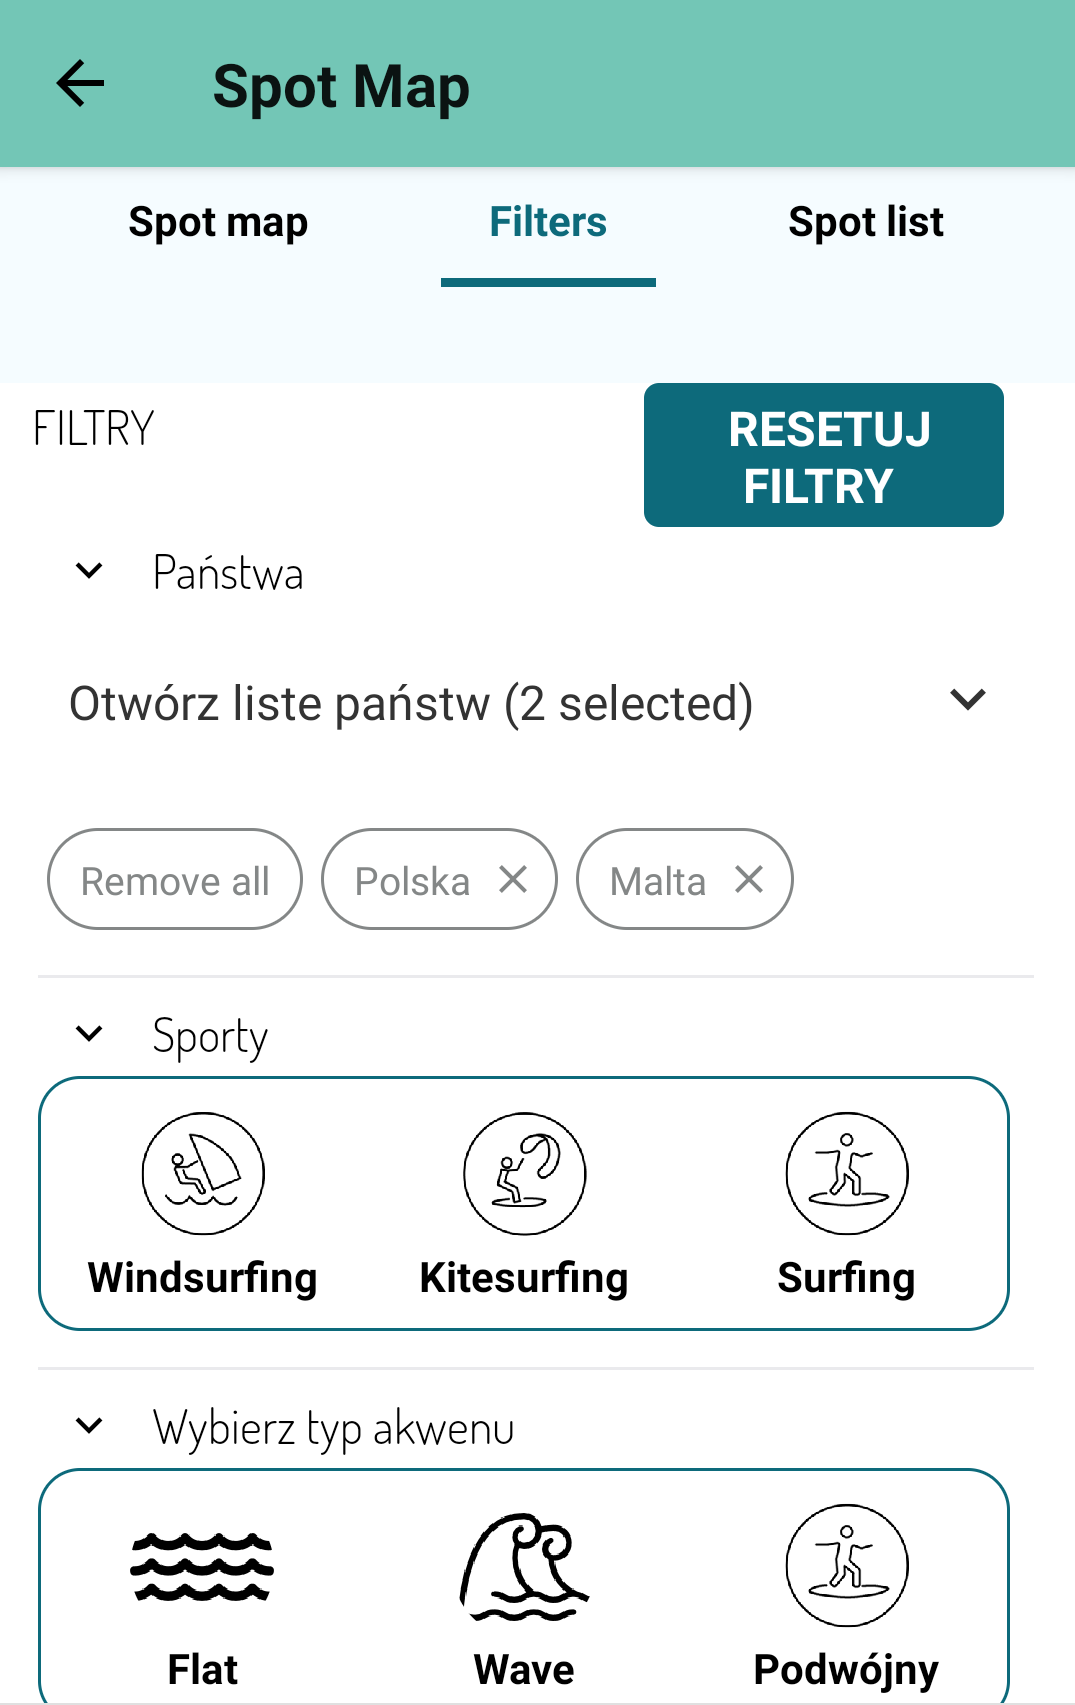
\includegraphics[width=0.45\textwidth]{img/mobile/filters-1}
	\end{center}
	\caption{...}
\end{figure}

\begin{figure}[h!]
    \begin{center}
        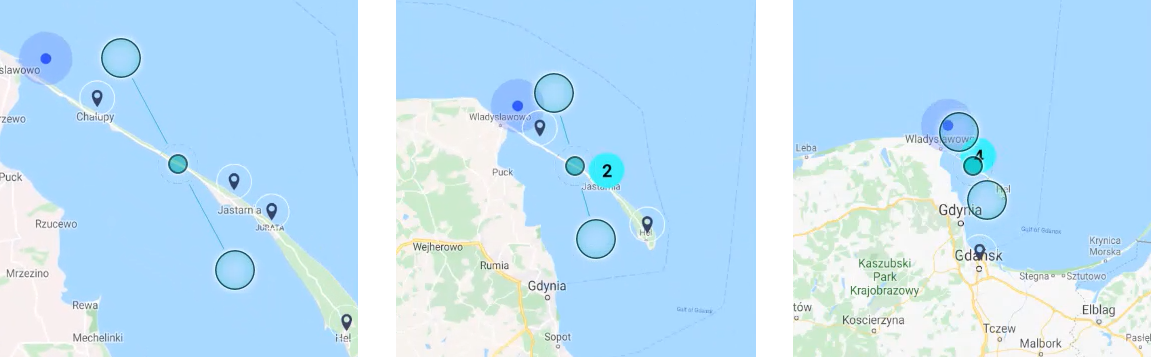
\includegraphics[width=1\textwidth]{img/mobile/clustering}
    \end{center}
    \caption{...}
\end{figure}




\chapter{Autoskalowanie}
\label{cha:autoscaling}

\cw{Cluster} SurfAdvisor skaluje się w dwóch wymiarach:

\begin{itemize}
    \item
    \cw{Pod} - \textbf{Horizontal Pod Autoscaling}\\
    ilość \cw{Pod}'ów \emph{(instancji)} danej aplikacji
    \item
    \cw{Node} - \textbf{Horizontal Node Autoscaling}\\
    ilość \cw{Node}'ów \emph{(wirtualnych maszyn)} składających się na \cw{Cluster}
\end{itemize} 

\section{Horizontal Pod Autoscaling}

Autoskalowanie \cw{Pod}'ów definiuje się poprzez skojarzony obiekt \cw{HorizontalPodAutoscaler}.
Kluczowe znaczenie mają właściwości:

\begin{itemize}
    \item
    minimalna ilość \cw{Pod}'ów
    \item
    maksymalna ilość \cw{Pod}'ów
    \item
    metryka, która wzbudza skalowanie
\end{itemize} 

Aby skalowanie było możliwe, definicja \cw{Pod}'a musi zawierać wymagania co do zużycia zasobów \emph{(CPU, RAM)}.

Działanie autoskalowania zaprezentowane zostanie podczas testu obciążeniowego \emph{dictionary-service}.
W stanie spoczynkowym liczba \cw{Pod}'ów tego \cw{Service}'u wynosi \textbf{1}, maksymalnie może osiągnąć \textbf{10}, 
skalowanie wzbudzane jest przekroczeniem \textbf{50\%} zużycia \textbf{CPU}.

\begin{figure}[!ht]
	\begin{center}
		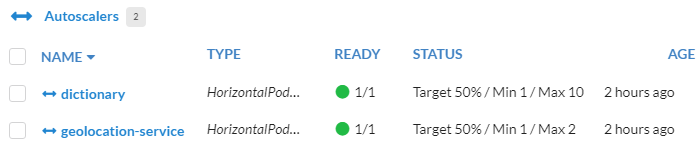
\includegraphics[width=0.9\textwidth]{img/autoscaling/hpa-autoscalers-normal}
	\end{center}
    \caption{Spoczynkowy stan Autoscaler'ów}
\end{figure}

\begin{figure}[!ht]
	\begin{center}
		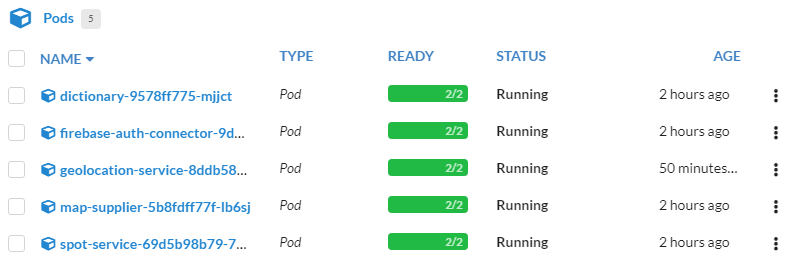
\includegraphics[width=0.9\textwidth]{img/autoscaling/hpa-pods-normal}
	\end{center}
    \caption{Spoczynkowy stan Pod'ów}
\end{figure}

W ramach testu obciążeniowego wysyłany jest za pomocą programu \emph{Postman} nieprzerwany szturm 10 tysięcy zapytań GET o treść jakiegoś słownika:

\begin{figure}[!ht]
	\begin{center}
		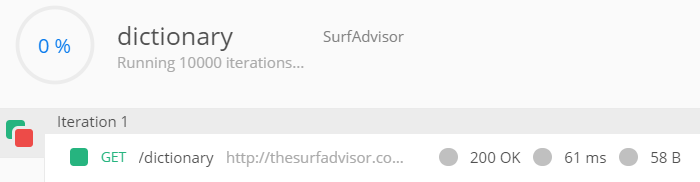
\includegraphics[width=0.8\textwidth]{img/autoscaling/hpa-dictionary-test-postman}
	\end{center}
    \caption{Test obciążeniowy \emph{dictionary-service} z Postmana}
\end{figure}

\cw{Autoscaler}'y reagują po około 10 sekundach zwiększając liczbę \cw{Pod}'ów \emph{dictionary-service}:

\begin{figure}[!ht]
	\begin{center}
		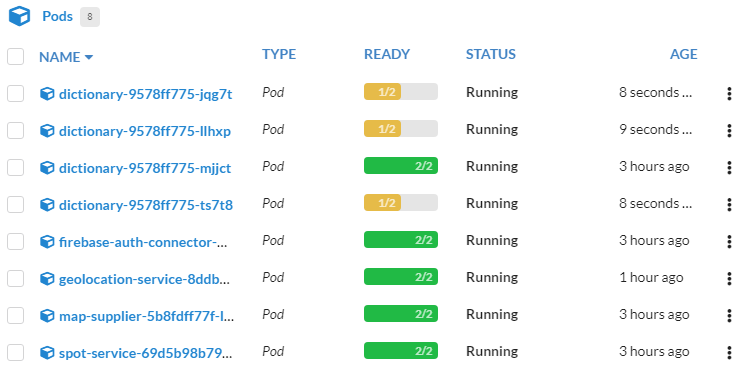
\includegraphics[width=0.9\textwidth]{img/autoscaling/hpa-pods-scale-up}
	\end{center}
    \caption{Stan Pod'ów przy skalowaniu w górę}
\end{figure}

\begin{figure}[!ht]
	\begin{center}
		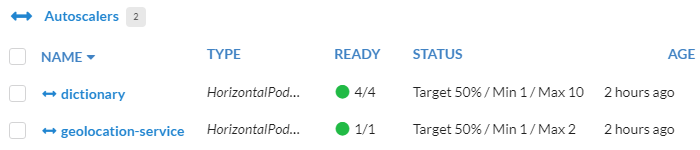
\includegraphics[width=0.9\textwidth]{img/autoscaling/hpa-autoscalers-scale-up}
	\end{center}
    \caption{Stan Autoscaler'ów przy skalowaniu w górę}
\end{figure}

Diagram poniżej pochodzi z konsoli webowej \emph{Grafana} - narzędzia, które wspólnie z \emph{Prometheus} umożliwiają śledzienie metryk technicznych \cw{Cluster}'a.
Przedstawione zostało zużycie CPU poszczególnych \cw{Pod}'ów podczas testu obciążeniowego:

\begin{figure}[!ht]
	\begin{center}
		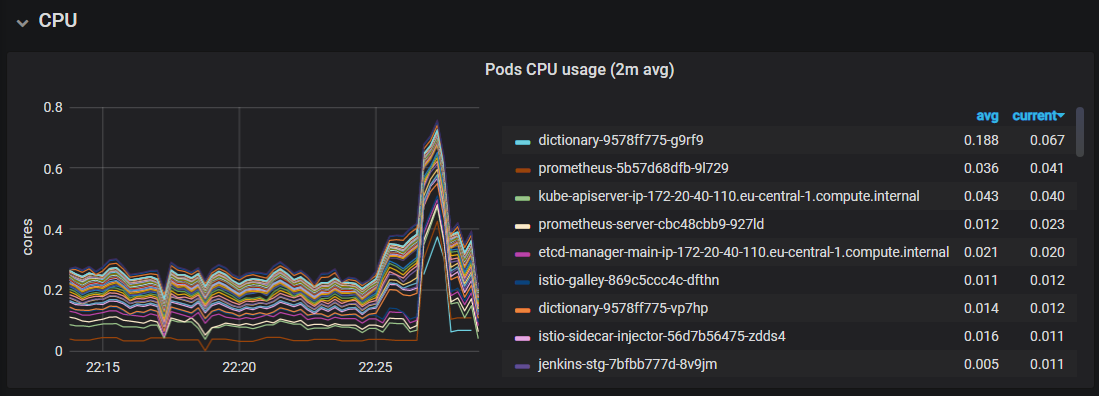
\includegraphics[width=1\textwidth]{img/autoscaling/hpa-grafana-scale-up}
	\end{center}
    \caption{Zużycie CPU podczas testu obciążeniowego \emph{dictionary-service}}
\end{figure}

\section{Horizontal Node Autoscaling}

Z kolei włączenie autoskalowania \cw{Node}'ów jest jeszcze prostsze. 
Ogranicza się do wdrożenia jednej z dostępnych online rekomendowanych definicji \cw{Service}'u \emph{cluster-autoscaler}.
Skalowanie pobudzane jest ilością \cw{Pod}'ów jakie Kubernetes próbuje wdrożyć.
Jeżeli istniejące \cw{Node}'y nie pomieszczą już więcej \cw{Pod}'ów, tworzone są kolejne.

Ilość instancji EC2 w stanie początkowym:

\begin{figure}[H]
	\begin{center}
		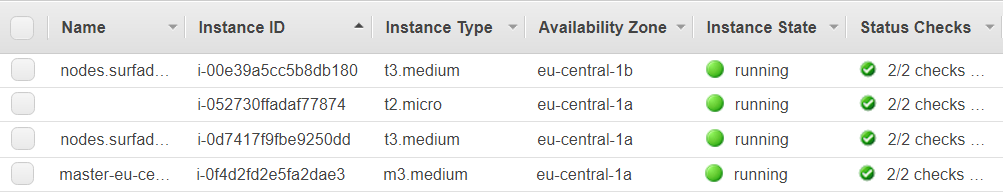
\includegraphics[width=1\textwidth]{img/autoscaling/ca-normal}
	\end{center}
    \caption{Spoczynkowy stan Node'ów}
\end{figure}

Poprzez manualne rozkazy zwiększania ilości \cw{Pod}'ów doprowadzono do przepełnienia \cw{Cluster}'a.
W logach \cw{Service}'u \emph{cluster-autoscaler} zarejestrowana jest reakcja na zastałą sytuację:

\begin{figure}[H]
	\begin{center}
		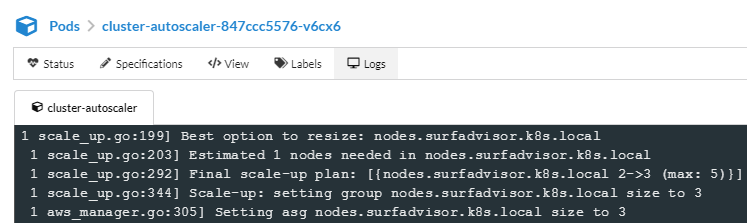
\includegraphics[width=0.9\textwidth]{img/autoscaling/ca-scale-up-logs}
	\end{center}
    \caption{Logi serwisu odpowiedzialnego za skalowanie horyzontalne Node'ów}
\end{figure}

Wynikiem tego działania jest uruchomienie dodatkowej instancji EC2, która rozszerzy pojemność \cw{Cluster}'a i umożliwi wdrożenie wszystkich \cw{Pod}'ów:

\begin{figure}[H]
	\begin{center}
		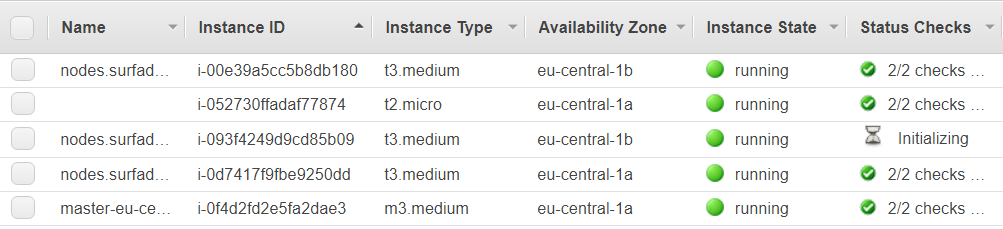
\includegraphics[width=1\textwidth]{img/autoscaling/ca-scale-up}
	\end{center}
    \caption{Stan Node'ów przy skalowaniu w górę}
\end{figure}

\chapter{Podsumowanie}
\label{cha:summary}



% itd.
% \appendix
% \include{dodatekA}
% \include{dodatekB}
% itd.

\printbibliography

\end{document}
